\documentclass[11pt,a4paper,ja=minimal,xelatex]{bxjsarticle}
\usepackage{zxjatype}
\usepackage{xeCJK}
\usepackage{fontspec}
\setmainfont{Times New Roman}
\setCJKmainfont{BIZ UDGothic}
\setCJKsansfont{BIZ UDGothic}
\setCJKmonofont{BIZ UDGothic}
\newcommand{\refmark}{{\fontspec{BIZ UDGothic}※}}  % ※はTimes New RomanにないためCJKフォントで表示
\usepackage{amsmath,amssymb}
\usepackage{graphicx}
\usepackage{booktabs}
\usepackage{tabularx}
\usepackage{url}
\usepackage{xurl} 
\usepackage{geometry}
\geometry{left=1.5cm,right=1.5cm,top=1cm,bottom=1cm,headheight=25pt,headsep=12pt}
\usepackage{fancyhdr}
\newcommand{\HeaderLeftIndent}{15pt}   % 左からの余白（例: 0pt, 1em, 5mm）。増やすと右に寄る
\newcommand{\HeaderVerticalShift}{7pt}% 上下のずれ。正で上に、負で下に（例: 3pt で上へ, -3pt で下へ）
% -------------------------------------------------
\pagestyle{fancy}
\fancyhf{}
\fancyfoot[C]{\thepage}
\fancyheadoffset[L]{\HeaderLeftIndent}
\fancyhead[L]{\raisebox{\HeaderVerticalShift}{\parbox[t]{\dimexpr\headwidth-1em\relax}{\fontsize{10.5}{13}\selectfont プロジェクト名: 潜在空間を用いたチャット型医薬品推奨ツール\\
提案者名: 川嶋宥翔}}}
\fancypagestyle{plain}{\fancyhf{}\fancyfoot[C]{\thepage}\fancyheadoffset[L]{\HeaderLeftIndent}\fancyhead[L]{\raisebox{\HeaderVerticalShift}{\parbox[t]{\dimexpr\headwidth-1em\relax}{\fontsize{10.5}{13}\selectfont プロジェクト名: 潜在空間を用いたチャット型医薬品推奨ツール\\
提案者名: 川嶋宥翔}}}\renewcommand{\headrulewidth}{0pt}}
\renewcommand{\headrulewidth}{0pt}
\newcommand{\SectionFontSize}{12}      % セクション見出し
\newcommand{\SectionBaseline}{10.5}       % セクション見出しの行送り
\newcommand{\SubsectionFontSize}{10.5}  % サブセクション見出し
\newcommand{\SubsectionBaseline}{10.5}    % サブセクション見出しの行送り
% 本文の文字サイズは \documentclass[11pt,...] の 11pt で指定（10pt/11pt/12pt などに変更可）
\newcommand{\BodyBaselineSkip}{11pt}  % 本文の行間
\newenvironment{bodyminipage}[2][c]{% [c|t|b], width
  \begin{minipage}[#1]{#2}%
  \setlength{\baselineskip}{\BodyBaselineSkip}%
  \setlength{\lineskip}{0.2em}%
}{\end{minipage}}
\usepackage{titlesec}
\titleformat{\section}{\fontsize{\SectionFontSize}{\SectionBaseline}\selectfont\bfseries}{\thesection}{0em}{}
\titleformat{name=\section,numberless}{\fontsize{\SectionFontSize}{\SectionBaseline}\selectfont\bfseries}{}{0em}{}
\titleformat{\subsection}{\fontsize{\SubsectionFontSize}{\SubsectionBaseline}\selectfont\bfseries}{\thesubsection}{0em}{}
\titleformat{name=\subsection,numberless}{\fontsize{\SubsectionFontSize}{\SubsectionBaseline}\selectfont\bfseries}{}{0em}{}
\titlespacing*{\section}{0pt}{1em}{0.25em}
\titlespacing*{\subsection}{0pt}{0.8em}{0.2em}
\usepackage{indentfirst}
\setlength{\parindent}{1em}
\usepackage{float}
\setlength{\intextsep}{3pt}      % 文中の float の上下の余白
\setlength{\textfloatsep}{2pt}   % ページ先頭・末尾の float と本文の余白
\usepackage{subcaption}
\captionsetup{font=small, justification=centering}
\captionsetup[subfigure]{font=footnotesize, justification=centering}
\usepackage{enumitem}
\usepackage{pifont}
\usepackage[draft=false,breaklinks]{hyperref}
\hypersetup{
    colorlinks=true,
    linkcolor=blue,
    citecolor=blue,
    urlcolor=blue
}

\author{}
\date{}

\begin{document}
\setlength{\baselineskip}{\BodyBaselineSkip}
\setlength{\lineskip}{0.2em}

\begin{center}
\fontsize{14}{17}\selectfont\bfseries
【提案プロジェクト詳細】
\end{center}

% ========== ① なにを作るか ==========
\section*{\ding{172} なにを作るか}

本提案が作るのは、チャットで症状を伝えるだけで、安心して市販薬を選べる医薬品推奨システムである。

\subsection*{背景（なぜ）}
ドラッグストアで、どの薬を選べばよいか迷った経験はないだろうか。棚には似た効能の製品が並び、どれが自分に本当に合う医薬品なのかと迷った経験は、多くの人が持っているはずだ。

私は現在、名古屋市内のドラッグストアで勤務している。現場では、耳が遠く説明を十分に聞き取れないご高齢の方、症状を日本語でうまく伝えられない外国人のお客様、多様な背景を持つ方々が「薬を選ぶ」という一点で困難に直面している。しかし現場は慢性的な人手不足にあり、繁忙時には一人ひとりに十分な時間を割くことができない。そのたびに、「もっと力になりたいのに」という無力感を覚えてきた。

この現場の葛藤は、個人だけの問題ではない。日本が直面する構造的課題と深く結びついている。

少子高齢化が進む日本では、医療機関の負担軽減が喫緊の課題である。その鍵を握るのが「セルフメディケーション」だ。これはWHOが「自らの健康に責任を持ち、軽度な不調は自分で手当てすること」と定義する概念である。実際、ドラッグストア業界の市場規模は拡大を続け、10兆円を超える産業へと成長している。しかし、その成長の裏には「場所の壁」と「知識の壁」という大きな2つの壁が存在する。

まず「場所の壁」だ。ドラッグストアは全国に広がっているが、その分布は均一ではない。特に過疎地では「相談できる店がない」という医療アクセス格差が生じている。図\ref{fig:dragstore}は、全国の都道府県別、および和歌山県内におけるドラッグストアの分布を示したものだ（経済産業省「商業動態統計」2020年、および筆者による調査）。私は和歌山県有田郡有田川町という、みかんで知られる町で生まれ育った。実家の近くにドラッグストアはなく、最寄り店舗までは約5km。車がなければ薬一つ買いに行けない環境だった。地図上の空白地帯は単なるデータではなく、かつての私や家族のように、薬へのアクセスに不安を抱える人々の生活がある。

\begin{figure}[H]
  \centering
  \begin{subfigure}[t]{0.32\textwidth}
  \centering
  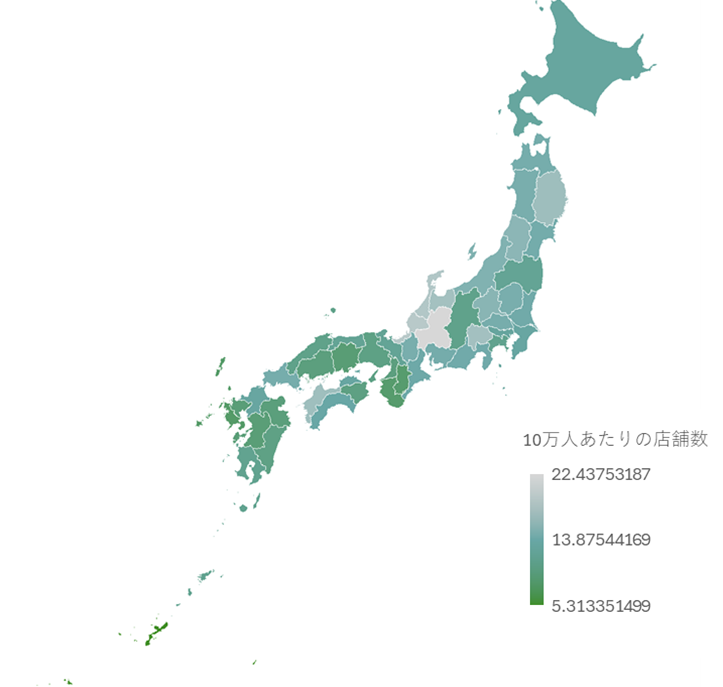
\includegraphics[width=\textwidth,keepaspectratio]{image/dragstore_injapan.png}
  \caption{都道府県別\\（経済産業省「商業動態統計」2020年）}
  \end{subfigure}
  \hfill
  \begin{subfigure}[t]{0.32\textwidth}
  \centering
  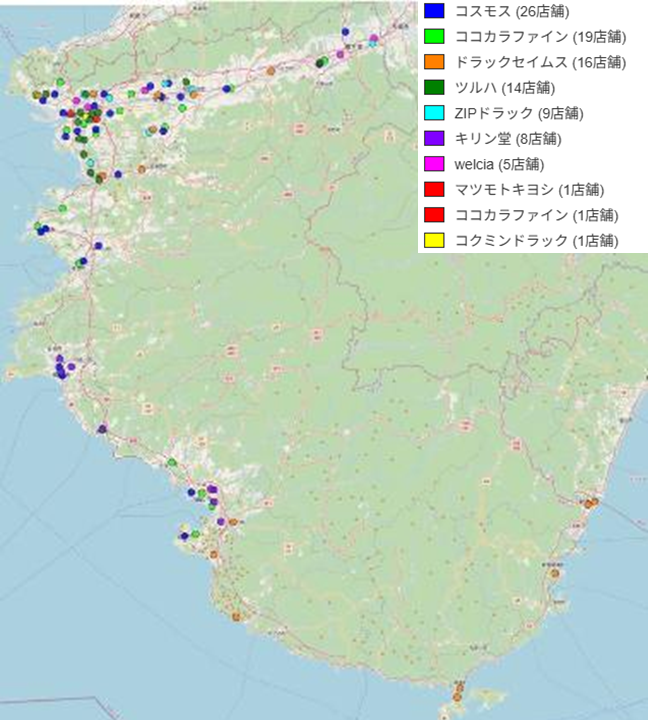
\includegraphics[width=\textwidth,keepaspectratio]{image/wakayama2.png}
  \caption{和歌山県における\\ドラッグストアの分布}
  \end{subfigure}
  \hfill
  \begin{subfigure}[t]{0.32\textwidth}
  \centering
  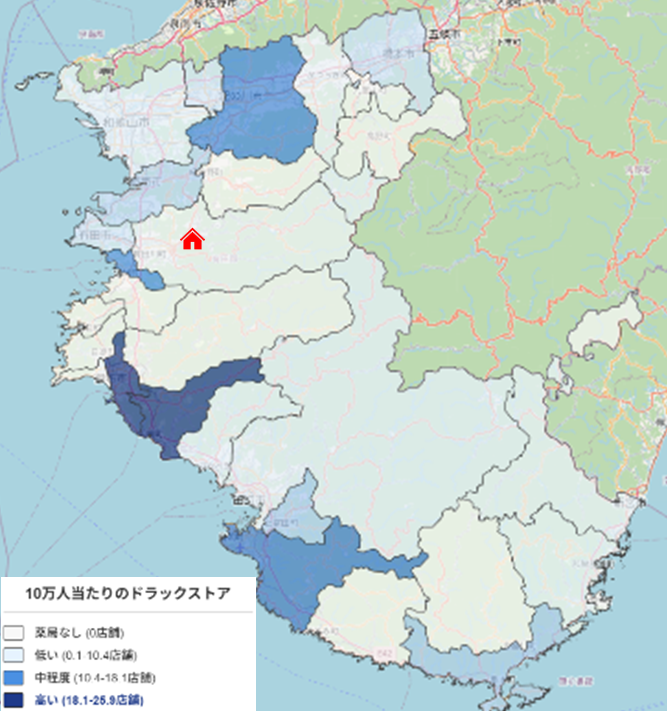
\includegraphics[width=\textwidth,keepaspectratio]{image/wakayama.png}
  \caption{人口10万人あたりの\\ドラッグストアの店舗数}
  \end{subfigure}
  \caption{ドラッグストアの地域分布}
  \label{fig:dragstore}
  \end{figure}

次に「知識の壁」である。たとえ店舗があっても、十分な専門人材が常に配置されているとは限らない。登録販売者や薬剤師の有効求人倍率は3倍を超え、慢性的な人材不足が続いている。さらに、薬機法の改正により一般用医薬品のインターネット販売が解禁され、利便性は向上した一方で、専門家の介在なしに誤った選択をしてしまうリスクも高まっている。実際、市販薬への依存や不適切使用(オーバードーズ)の問題は深刻化している。

つまり、日本では今、セルフメディケーションが求められているにもかかわらず、相談できる場所も、常に頼れる知識も、十分に行き渡っていないという構造的矛盾が存在している。

だからこそ私は、この「場所の壁」と「知識の壁」をテクノロジーで取り払い、誰もが、住む地域や言語、時間帯に関係なく、「どこでも・安心して」最適な医薬品を選択できる社会を実現する。それが本プロジェクトの出発点である。

\newpage
\subsection*{目的・目標（何を・どこまで）}

\noindent\textbf{■ 目的（何を）}

本提案の\textbf{目的}は、「場所の壁」と「知識の壁」がもたらす医薬品の選びにくさを解消し、\textbf{誰もが「どこでも・安心して」医薬品を選択できる}社会に貢献することである。そのために、症状を入力するだけで、体質や症状に合った医薬品を推奨するチャットツールを開発する。

\vspace{0.3em}
\noindent\textbf{■ 現状のシステム（実装・本番運用済み）}

\noindent
\begin{bodyminipage}[c]{0.75\textwidth}
すでに以下の機能を実装し、右のQRコードでWebアプリを公開している。

\begin{itemize}[nosep,leftmargin=1.5em]
  \item \textbf{推奨エンジン}：症状文をLLMで解析（NLU）し、その結果に基づきルールベースのスコアリング（症状適合度・副作用リスク・年齢適合性・用法簡便性・相互作用リスク・ボーナス・ペナルティの7要素）で医薬品を評価して上位3件を推奨（推奨判断はルールベース、症状理解にLLMを利用）
  \item \textbf{5層防御}（入力検証・NLU・禁忌・アレルギー・最終判定）：各層を通過した場合にのみ推奨を返し安全性を担保している。禁忌判定99\%以上・アレルギー98\%除外を達成（年齢・妊娠・授乳・既往症・アレルギー成分の組み合わせを網羅した独自テストケース300件による測定値）
  \item \textbf{4言語対応}（日・英・中・韓）：訪日外国人・在留外国人にも対応
  \item \textbf{管理者インターフェース}：AIによる自動応答・手動介入・監視機能
\end{itemize}
\end{bodyminipage}\hfill
\begin{minipage}[c]{0.22\textwidth}
\centering

\includegraphics[width=\linewidth,keepaspectratio]{image/Demo.png}
\captionof{figure}{本システムのデモ（\url{https://medicine.yutok.dev/}）}
\end{minipage}

\noindent
\begin{bodyminipage}[c]{0.62\textwidth}
\noindent\textbf{■ 未踏期間の目標（どこまで作るか）}

現状の限界は二点ある。一点目は、症状解析にLLMを用いている一方で\textbf{スコアリングはルールベースのみ}で行っているため、症状表現の揺れや多様な言い回しをスコアに十分反映しきれない推奨精度上の限界。二点目は、推奨結果が\textbf{文章中心の表示}であり（図\ref{fig:medicine_recommended}）、複数の推奨医薬品を並べて比較・識別することが利用者にとって難しいというUI上の課題である。

未踏期間中に\textbf{潜在空間ベクトル類似度モジュール}を新たに実装・既存システムに統合し、ルールと潜在空間のハイブリッドスコアリングにより推奨精度を向上させる。あわせて、推奨結果の表示を右のような\textbf{カルーセル型UI}へ変更し、利用者が推奨医薬品を画像を用いて直感的に識別できるようにする。図\ref{fig:carousel-ui}はWebアプリ版カルーセルUIの実装イメージであり、図\ref{fig:line-image}はLINE版での実装イメージである。これにより、\textbf{利用者の理解促進と安心感の向上}を図る。なお、未踏期間中の商品画像に関しては、代表的な製品を中心に手動登録による検証を進める。

表\ref{tab:roadmap}に現状と未踏期間の実装内容の対比を示す。開発の到達目標は、ルールと潜在空間によるハイブリッドスコアリングの実装と、利用者が直感的にわかりやすいUIの実装を完了することである（詳細な開発線表は\ding{175}に示す）。

\end{bodyminipage}
\hfill
\begin{minipage}[c]{0.35\textwidth}
\centering
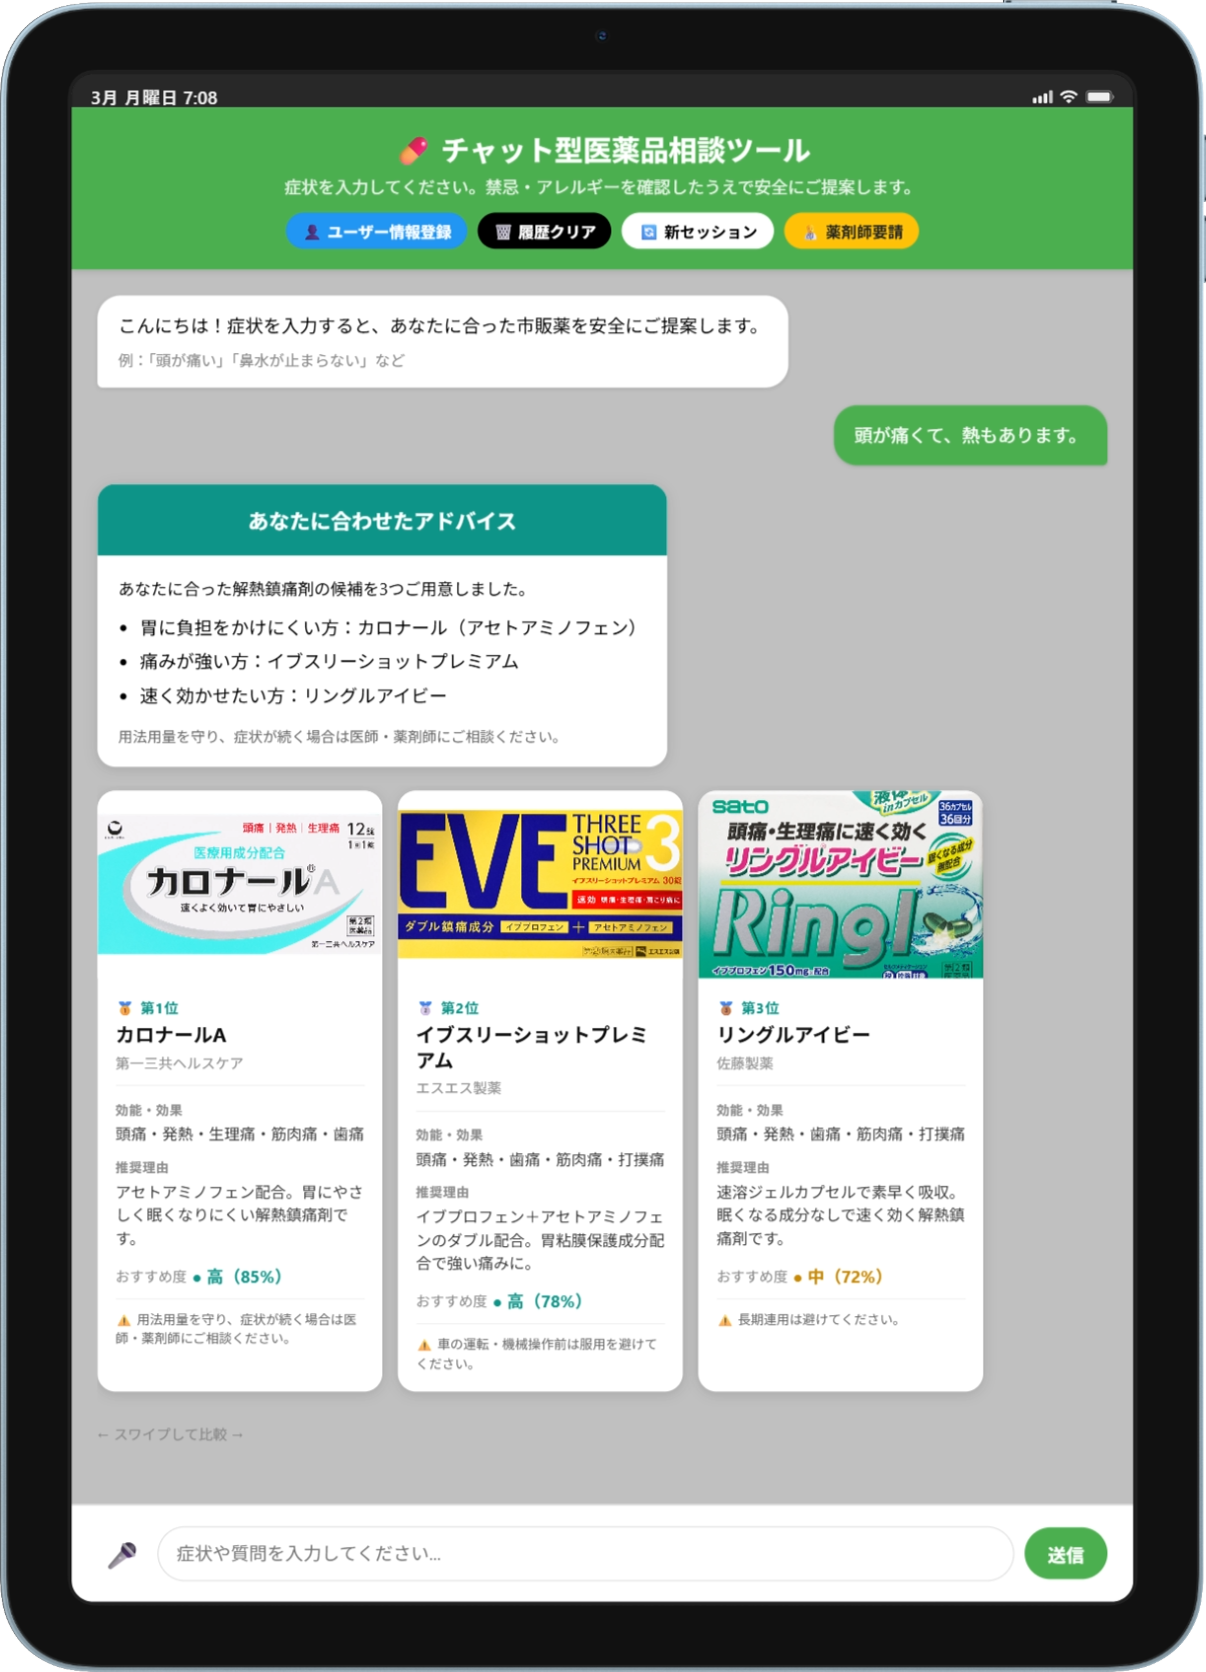
\includegraphics[width=\linewidth,keepaspectratio]{image/carousel_webui.png}
\captionof{figure}{Webアプリ版カルーセルUI(例)}
\label{fig:carousel-ui}
\end{minipage}

\begin{table}[H]
\centering
\caption{現状と未踏期間の実装対比}
\label{tab:roadmap}
\small
\begin{tabularx}{\textwidth}{|l|X|X|}
\hline
\multicolumn{1}{|c|}{\textbf{項目}} & \multicolumn{1}{c|}{\textbf{現状（実装済み）}} & \multicolumn{1}{c|}{\textbf{未踏期間で実装}} \\
\hline
推奨エンジン & LLMによる症状解析＋スコアリング & 潜在空間を統合したハイブリッドスコアリング \\
\hline
安全性指標 & 禁忌判定99\%以上・アレルギー98\%除外 & 安全性指標を維持したまま統合・安全性検証レポート作成 \\
\hline
言語対応 & 4言語（日・英・中・韓） & 維持 \\
\hline
推奨精度 & ルールベーススコアリング（表記揺れに一部限界） & 潜在空間統合により精度向上 \\
\hline
表示UI & 文章中心の推奨（候補の比較・識別が難しい） & カルーセル型UI（医薬品画像表示）視覚的な比較を可能にする \\
\hline
\end{tabularx}
\end{table}

\vspace{0.3em}
\noindent\textbf{■ システム概要}

本提案で作るのは、自然言語で症状を入力すると、自身の体質や症状に合った医薬品を推奨するシステムである。既存の推奨システムを土台に、潜在空間を統合したハイブリッドスコアリングにより、推奨精度の向上を目指す。LLMは症状抽出（NLU）に限定し、推奨判断はルールと潜在空間のハイブリッドで行うため、安全性を数学的に保証できる。

\noindent\textbf{【潜在空間とは】}　潜在空間とは、単語や文章を数値ベクトルに変換した多次元の意味空間である。「頭が痛い」「頭痛がする」のように表記が異なっても、意味的に近い表現は空間上で近い位置に配置される性質を持つ。本システムでは、ユーザーの症状記述と医薬品それぞれを同じ潜在空間上に変換し、その距離を用いて「どの医薬品がユーザーの症状に最も効果的か」を定量的に評価する。これにより、ルールベースでは対応しきれない症状表現の揺れや多様な言い回しにも対応できる。医薬品はPMDA（独立行政法人医薬品医療機器総合機構）が公開する添付文書情報をもとに独自に構築したもので、約10,000品目を収録している。

図\ref{fig:flowchart}に本アプリケーションの処理フロー全体を示す。医薬品推奨に至る経路では\textbf{5層防御}を採用し、各層の通過条件を満たした場合にのみ推奨結果を返すことで安全性を担保する。

\begin{figure}[H]
\centering

\includegraphics[width=\textwidth,keepaspectratio]{image/flowchart.png}
\caption{医薬品相談AIシステム - 処理フロー全体}
\label{fig:flowchart}
\end{figure}

5層防御は、実装の時系列に沿って次の6段階である。(1)入力検証（Layer1）：セキュリティリスク評価とユーザー属性抽出。(2)入力分類：入力を分類し、医薬品推奨に進むか医師相談・質問応答等に振り分ける。(3)NLU（症状抽出）（Layer2）：入力から症状集合へ変換。(4)禁忌チェック（Layer3）：年齢・妊娠・授乳・既往症等に基づきリスクが高い場合は医師受診を促し推奨しない。(5)医薬品候補の取得・アレルギー除外（Layer4）：禁忌・アレルギー該当品をスコアリング前に除外。(6)スコアリング・最終判定（Layer5）：上位$k$件（$k=3$）を推奨し、不足情報があれば質問を生成する。

\vspace{0.3em}
\noindent\textbf{■ 補足（UI・運用面）}

\textbf{薬剤師要請}：図\ref{fig:medicine_recommended}のように薬剤師要請ボタン（黄色）を常時表示しており、利用者がいつでもシームレスに相談を専門家へ切り替えられるようにしている。

\textbf{管理者画面}：図\ref{fig:admin}に示す管理者画面では、自動応答の有無、管理者によるチャットでの医薬品に関する質問応答、推奨医薬品のスコアリング計算フロー、ユーザー属性情報の確認が可能である。

\textbf{入力分類（トリアージ）の補足}：LLMにより入力をEmergency/Emotional/Physical/Ask/Otherに分類する。\textbf{Emergency}のときは医師相談推奨・救急案内で処理を停止する。診断名が含まれる場合も医師相談推奨を返し薬推奨には進まない。\textbf{Ask}は医薬品に関する質問フローであり、用法用量・効能・ドーピングの該当性などの質問に対応する。\textbf{Other}は店舗案内・遺失物・質問応答等である。\textbf{Emotional}はカウンセリング応答であり、心の不調や睡眠薬などの高リスク医薬品に対応する。なお、Emotionalにおいてユーザーが医薬品を希望する場合は医薬品の推奨を可能としている。\textbf{Physical}は症状の入力の場合に医薬品推奨パス（(3)NLU以降）に進む。

\begin{figure}[H]
\centering
\begin{minipage}[t]{0.38\textwidth}
  \centering
  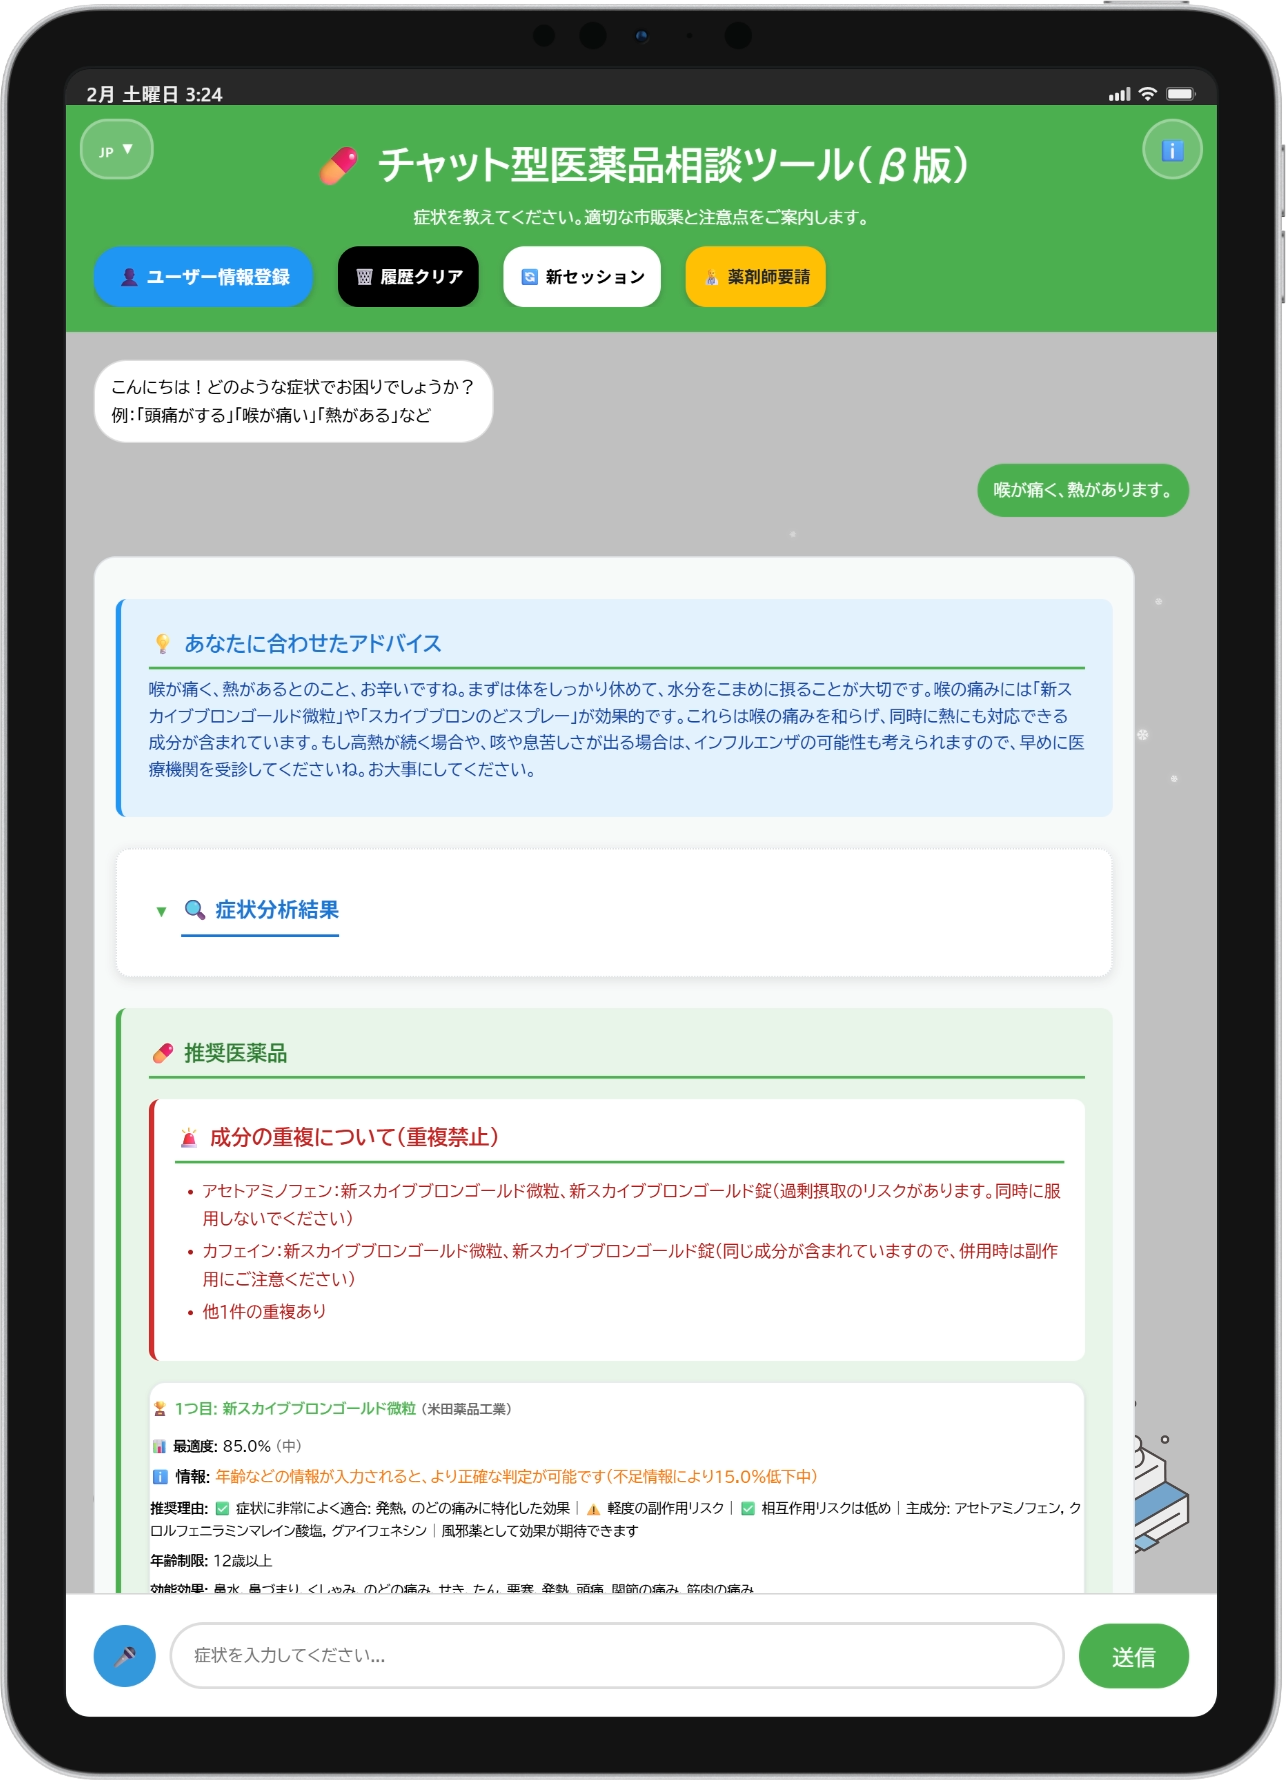
\includegraphics[width=\textwidth,keepaspectratio]{image/medicine_recommended.png}
\end{minipage}
\hfill
\begin{minipage}[t]{0.58\textwidth}
  \centering
  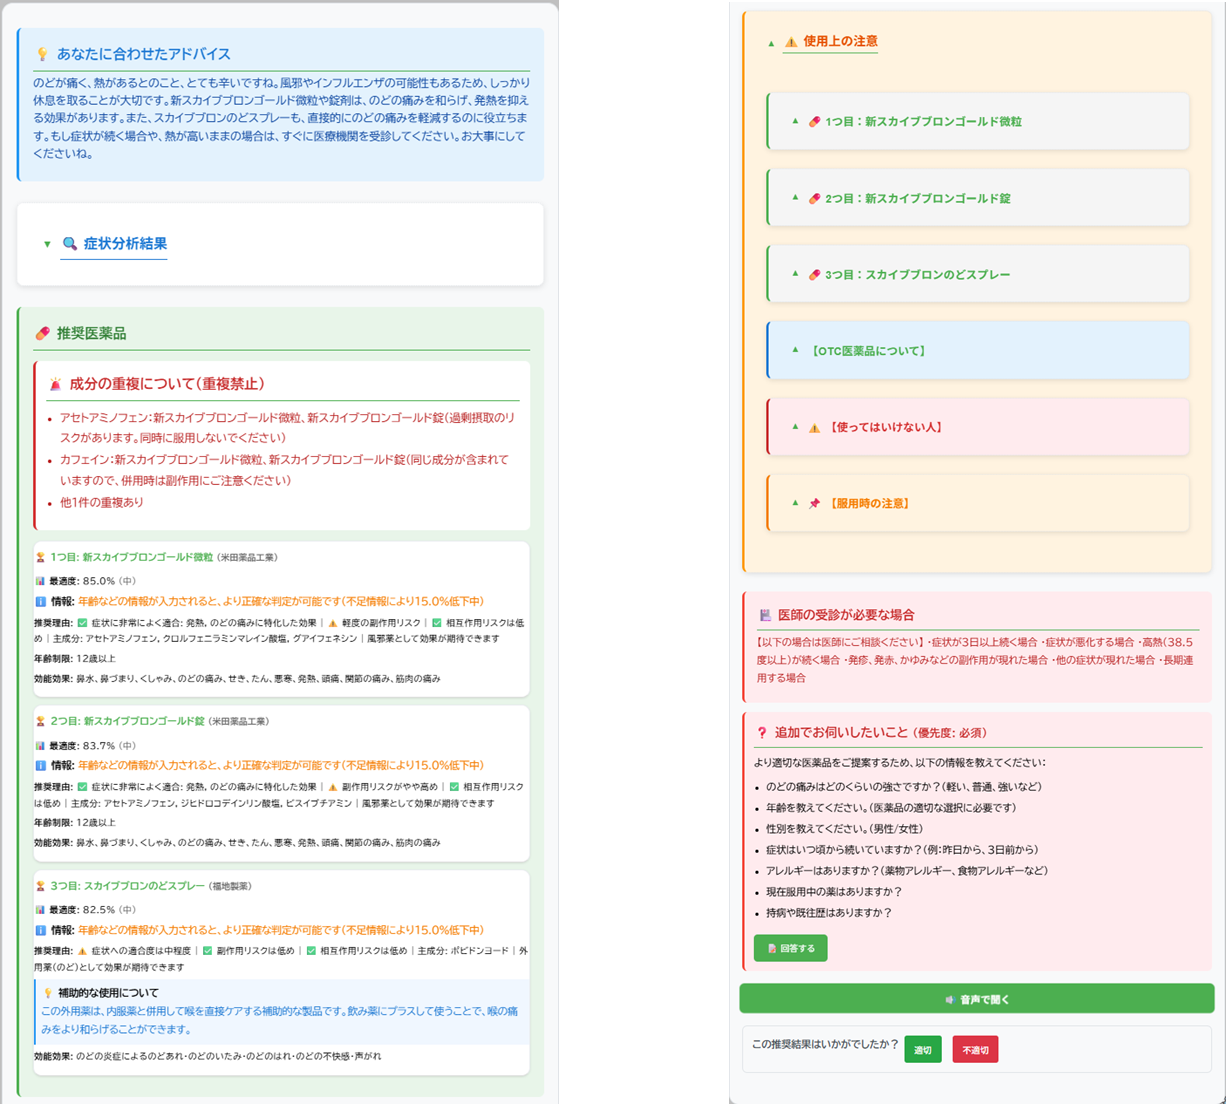
\includegraphics[width=\textwidth,keepaspectratio]{image/recommend.png}
\end{minipage}
\caption{推奨結果の表示例（左：アドバイス・症状分析・推奨医薬品・成分重複注意、右：推奨結果の全文）}
\label{fig:medicine_recommended}
\end{figure}

\begin{figure}[H]
\centering
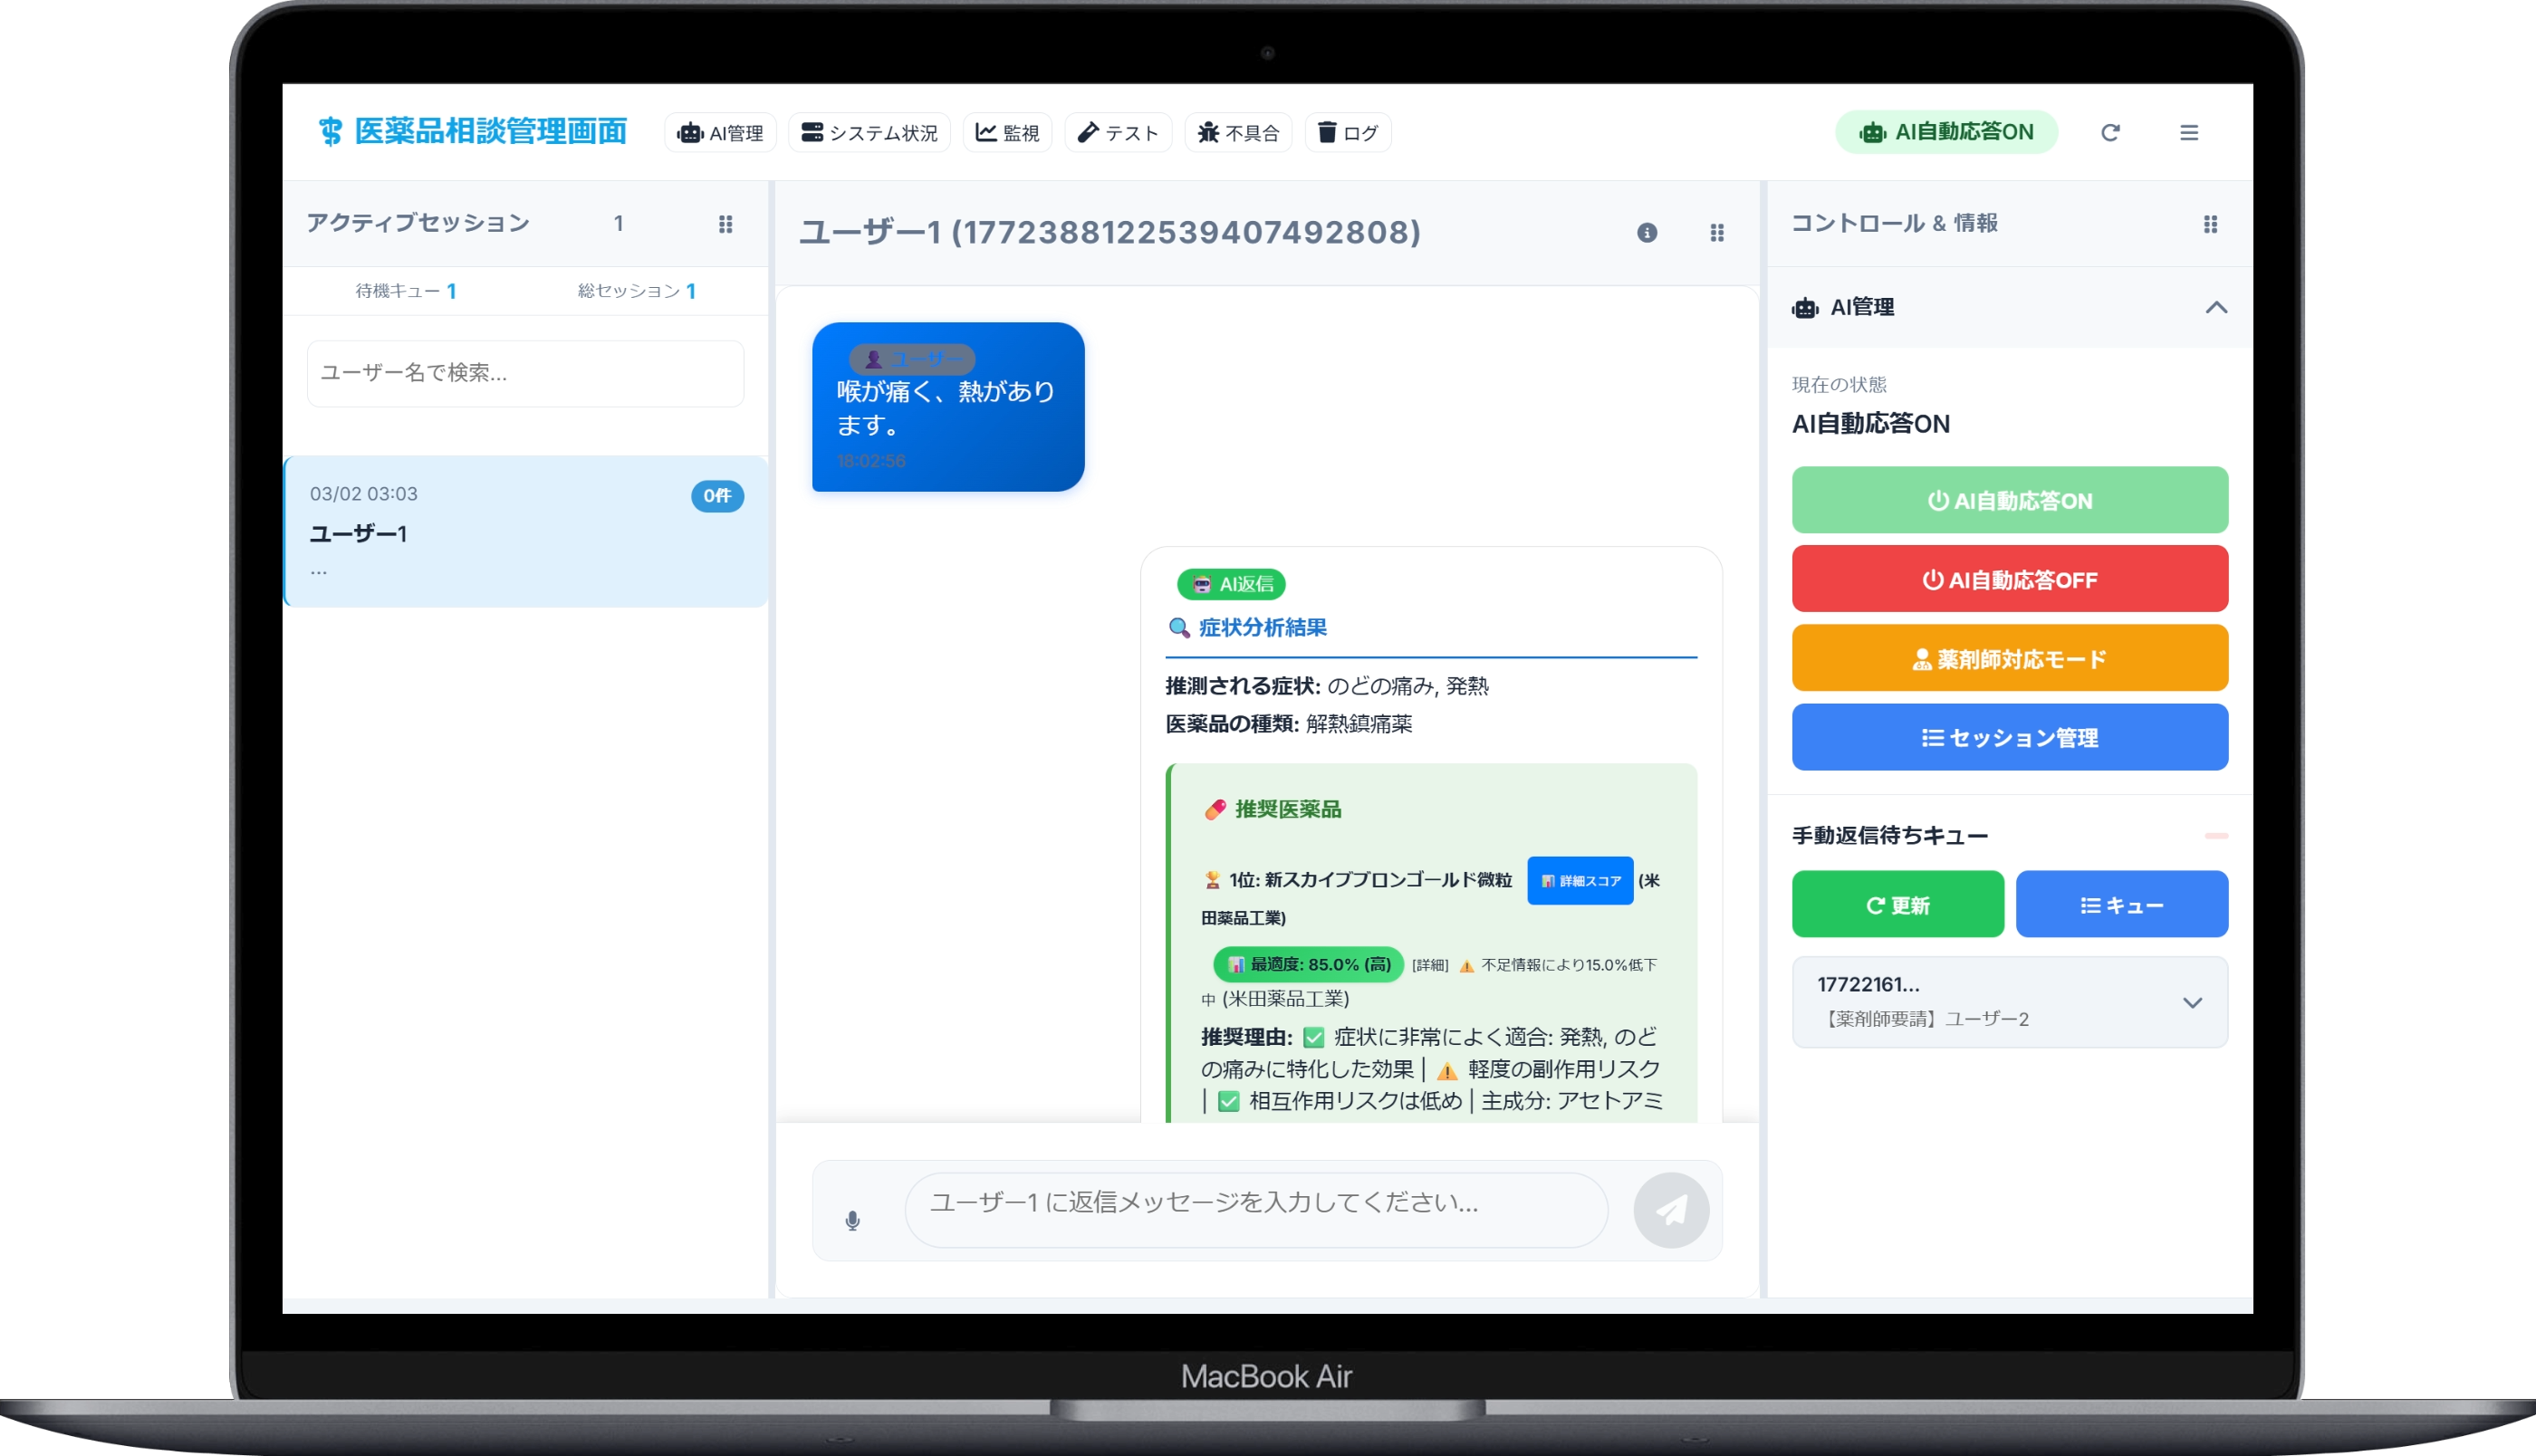
\includegraphics[width=0.6\textwidth,keepaspectratio]{image/admin.png}
\caption{管理者画面（AIによる自動応答・手動返信・監視・介入機能）}
\label{fig:admin}
\end{figure}

% ========== ② どんな出し方を考えているか ==========
\section*{\ding{173} どんな出し方を考えているか}

開発したシステムの社会実装は、短期・中期・長期の三段階で進める。

\textbf{短期（未踏期間中～修了直後）}は、相談補助ツールとしてWebアプリの無料公開を継続し、実利用環境での検証を行う。同時に、薬剤師・登録販売者による監修を並行して実施し、推奨ロジックと安全性の妥当性を専門家の視点から検証・改善する。利用者フィードバックと専門家監修の両輪で改善サイクルを回すことで、実運用に耐えうる信頼性を確立する。

\textbf{中期（〜1年）}には、LINE Messaging APIを活用したLINE公式アカウントを公開し（図\ref{fig:carousel-all}右）、チャット形式で気軽に相談できる環境を整備する。さらに、Yahoo!ショッピング商品検索APIを活用し、すべての推奨医薬品のパッケージ画像をリアルタイム取得・表示するビジュアル推奨機能を実装する。視覚的提示により、利用者の理解促進と安心感の向上を図る。あわせて、技術のOSS化を検討し、外部検証を受ける体制を整える。情報処理学会や医療情報学関連学会での発表も視野に入れ、技術的妥当性と社会的意義の両面で評価を獲得する。

\textbf{長期（〜3年）}は、未踏アドバンスト等の枠組みを活用し、ドラッグストア向けSaaSやAPI提供としての実用化を目指す。画像基盤については、製薬メーカーと直接交渉を行い、外装・内装・剤形を含む自前の医薬品画像データベースの構築を目指す。これによりEC系APIへの依存を脱却し、規約制約を受けない安定運用を実現する。エンドユーザー向けには無料利用を維持しつつ、店舗向けSaaS等による持続可能なビジネスモデルへと展開する。

本プロジェクトは、単なるアプリ公開にとどまらない。技術的妥当性、専門家監修、制度対応、ビジネス持続性を段階的に積み上げながら、社会基盤として定着させることを最終目標としている。

% ========== ③ 斬新さの主張・期待される効果 ==========
\section*{\ding{174} 斬新さの主張・期待される効果}

\subsection*{既存調査に基づく位置づけ}

医薬品の相談手段としては、ドラッグストアや薬局で薬剤師・登録販売者に直接相談する方法が一般的であり、近年ではオンライン診療や遠隔服薬指導などの医療サービスも普及しつつある。しかしこれらは安心感が高い一方で、移動・待ち時間や予約の手間があり、軽度の体調不良など日常的な場面では気軽に利用しづらい場合が多い。

手軽さを求めて、インターネット検索や生成AIによる症状相談が利用されることも増えているが、生成AI等を用いた医療相談には、推奨根拠の不透明性、禁忌・アレルギー判定の保証不足、ハルシネーションによる誤情報など、安全性の観点で看過できない課題がある。

こうした背景を受け、OTC医薬品に特化した相談サービスも存在する。代表例として、症状選択型問診のUbie、漢方特化のYOJO、企業向け健康相談のDカウンセラーneoなどが挙げられる。これらは固定問診・キーワードマッチ・特定領域への特化といった方式が多く、自然言語で多様な症状を柔軟に扱う対話型としての汎用性には限界がある。

図\ref{fig:competition}に既存サービスと本提案の比較を、図\ref{fig:positioning}に「安全性」と「汎用性」の二軸によるポジショニングマップを示す。本提案では、チャット型インターフェースによる柔軟な入力と潜在空間を用いた医薬品スコアリングを組み合わせ、高安全性と高汎用性の両立を目指す。

\begin{figure}[H]
\centering
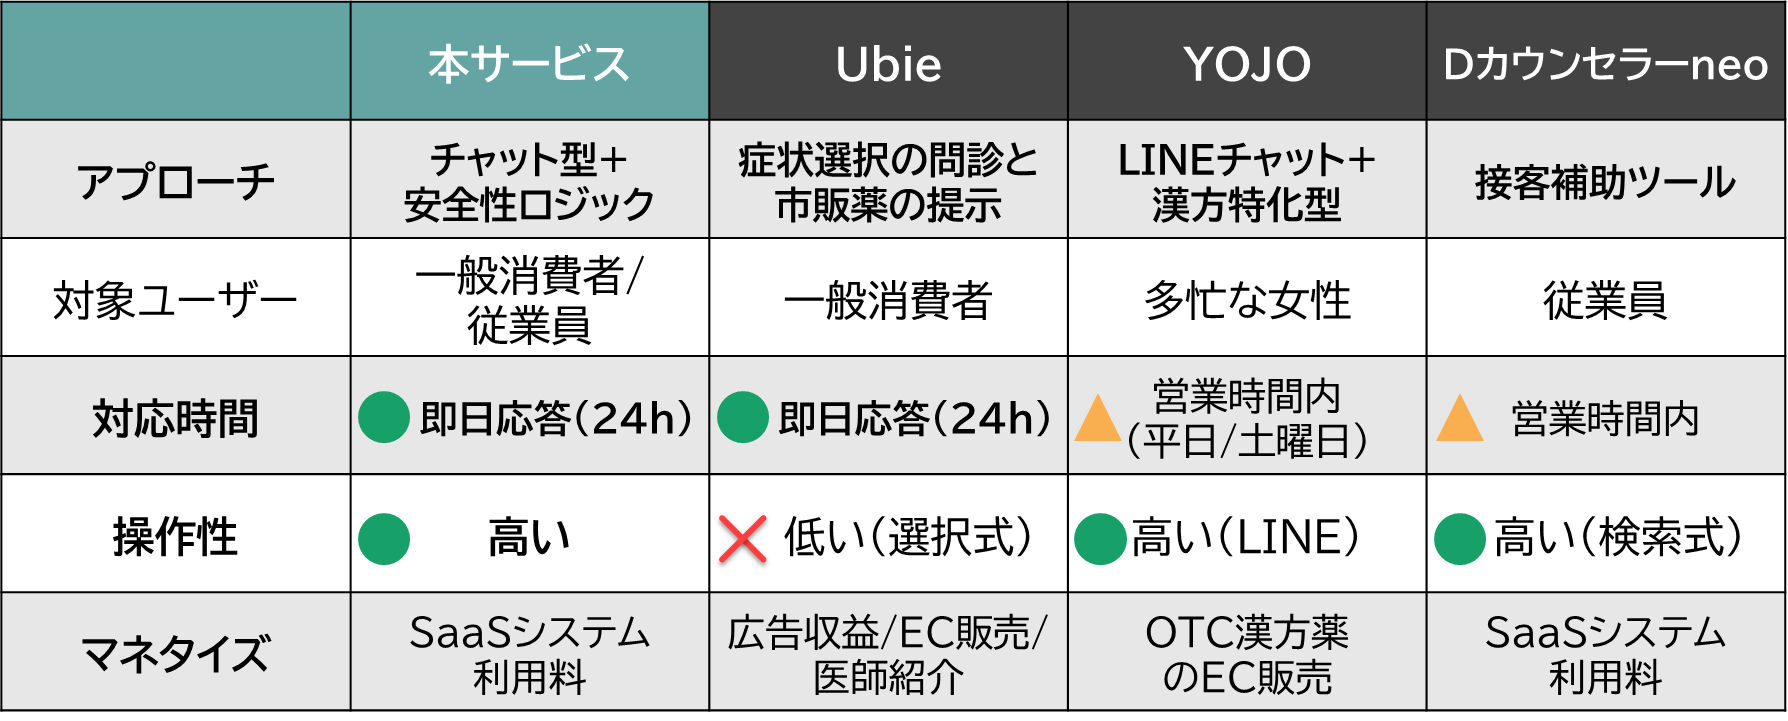
\includegraphics[width=0.6\textwidth,keepaspectratio]{image/competition.png}
\caption{競合との比較}
\label{fig:competition}
\end{figure}

\begin{figure}[H]
\centering
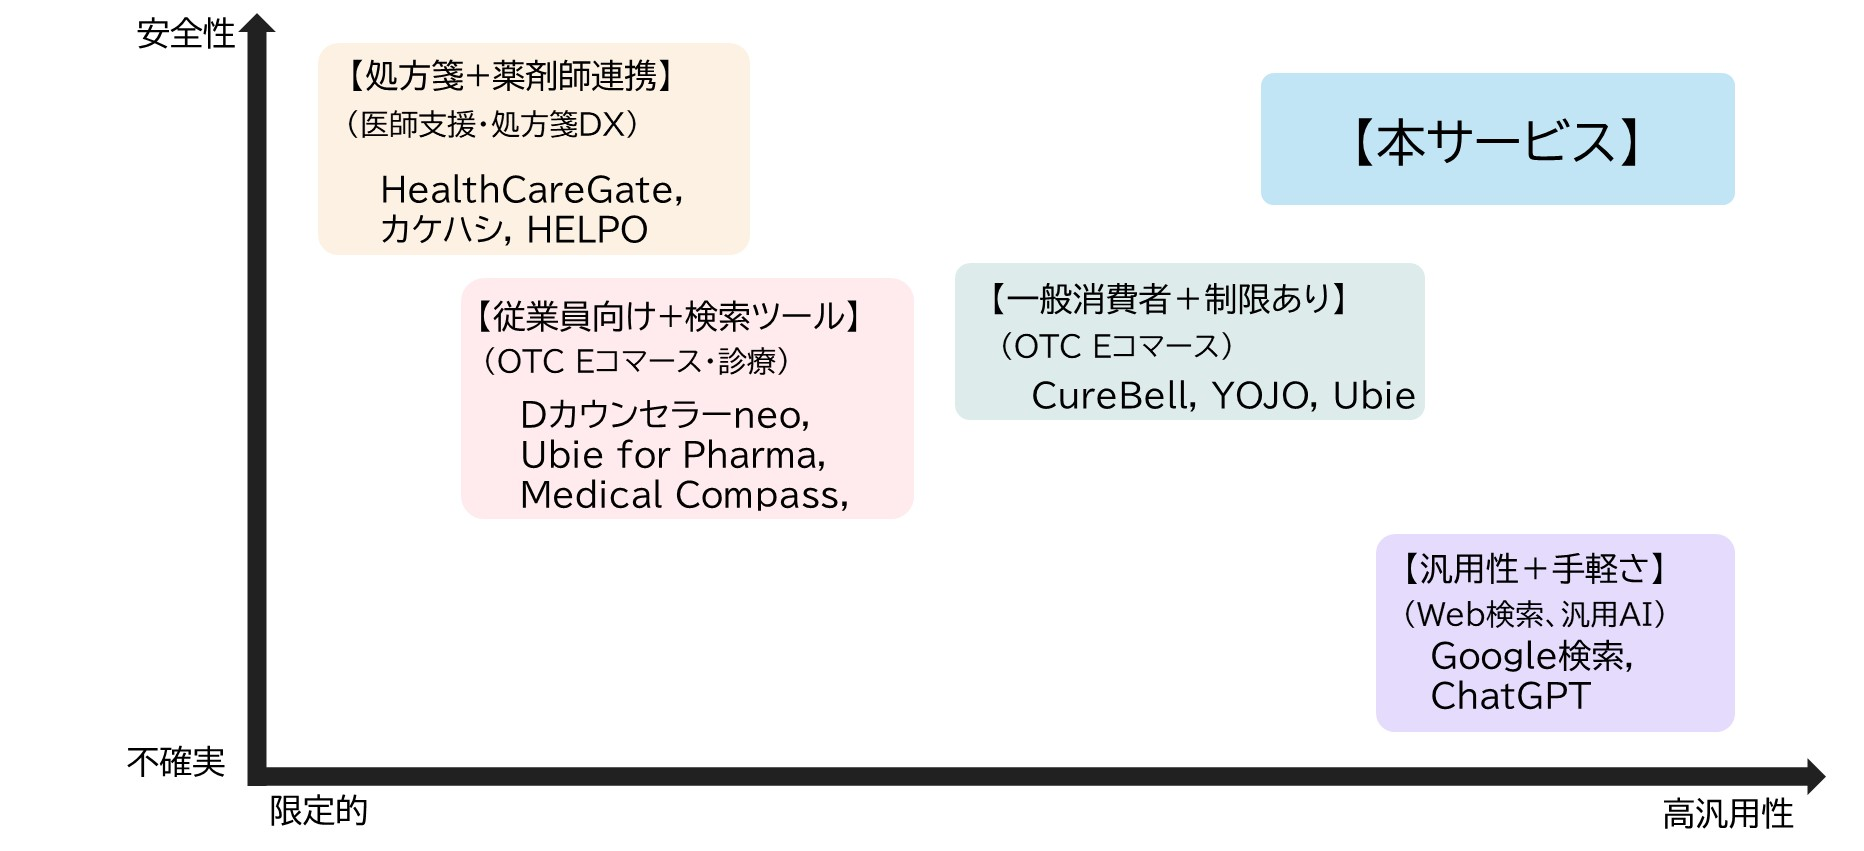
\includegraphics[width=0.6\textwidth,keepaspectratio]{image/positioning_map.jpg}
\caption{ポジショニングマップ（安全性×汎用性）}
\label{fig:positioning}
\end{figure}

以上を技術的に整理すると、生成AIは自然言語理解に優れる一方で安全性の保証が難しく、純粋なルールベースは透明性・安全性が高いものの症状表現の多様性に弱い。現状のOTC相談ツールの多くはキーワードマッチや選択式に依存しており、ユーザーの症状を十分に反映した推奨には至っていない。

本提案では、判断を機械に丸投げせず、禁忌・アレルギー等のリスクをルールで先に除外した上で、説明可能な形で医薬品を推奨する。LLMの役割を自然言語理解（症状抽出）に限定し、推奨判断はルールベースと潜在空間ベクトル類似度のハイブリッドで行う。具体的には、入力検証・NLU・禁忌・アレルギー・最終判定の5層をすべて通過した場合にのみ推奨が成立し、潜在空間の類似度はユーザーの体質に合った候補へのスコア付けにのみ用いるため、安全性が担保される。スコアリングでは、症状と医薬品の意味的類似度$\mathrm{sim}(v_u, v_m)$（潜在空間ベクトルのコサイン類似度）を既存の7要素スコアと統合し、信頼度に応じた動的重みで曖昧な入力時は潜在空間をやや重視する設計とする。その結果、自然言語入力の柔軟性を保ちつつ、利用者が推奨内容を理解した上で安心して選択できる医薬品推奨を実現する。なお、本システムの法的位置づけについては、名古屋市健康福祉局生活衛生部環境薬務課および愛知県医薬安全課監視グループに照会し、「診断を行わないためSaMD（医療機器ソフトウェア）に該当しない」との見解を得ている（正式な厚生労働省判断ではなく行政窓口への確認であることを明記する）。OTCの範囲を超えるケースでは推奨を止め医師・薬剤師への案内を行う設計としており、医師法・薬剤師法上の診断・調剤行為には一切関与しない。あわせて、音声入力・音声読み上げやオンボーディングガイド（図\ref{fig:onboarding}）、日本語・英語・中国語・韓国語の4言語対応（図\ref{fig:language}）により、高齢者や訪日・在留外国人にも利用しやすいアクセシビリティを確保している。

さらに、技術的差別化に加えてプラットフォーム面での差別化も図る。未踏修了後には、LINE Messaging APIを活用し、日常的に利用するLINE上で完結する医薬品相談サービスとして展開する計画である（図\ref{fig:carousel-all}）。LINEは国内月間アクティブユーザーが約1億人（人口の約85\%）にのぼり、専用アプリの追加インストールが不要な点が利点である。カルーセル形式で、医薬品のパッケージ画像・商品名・効能・推奨理由をカードとして提示し、ユーザーはスワイプ操作で自身に合った複数の医薬品を直感的に比較できる。また、継続的なフォローや薬剤師への相談連携も想定しており、誰もがどこでもまるで専門家が隣にいるように安心して医薬品を選び購入できる基盤を目指す。

\begin{figure}[H]
\centering
\begin{subfigure}[t]{0.45\textwidth}
  \centering
  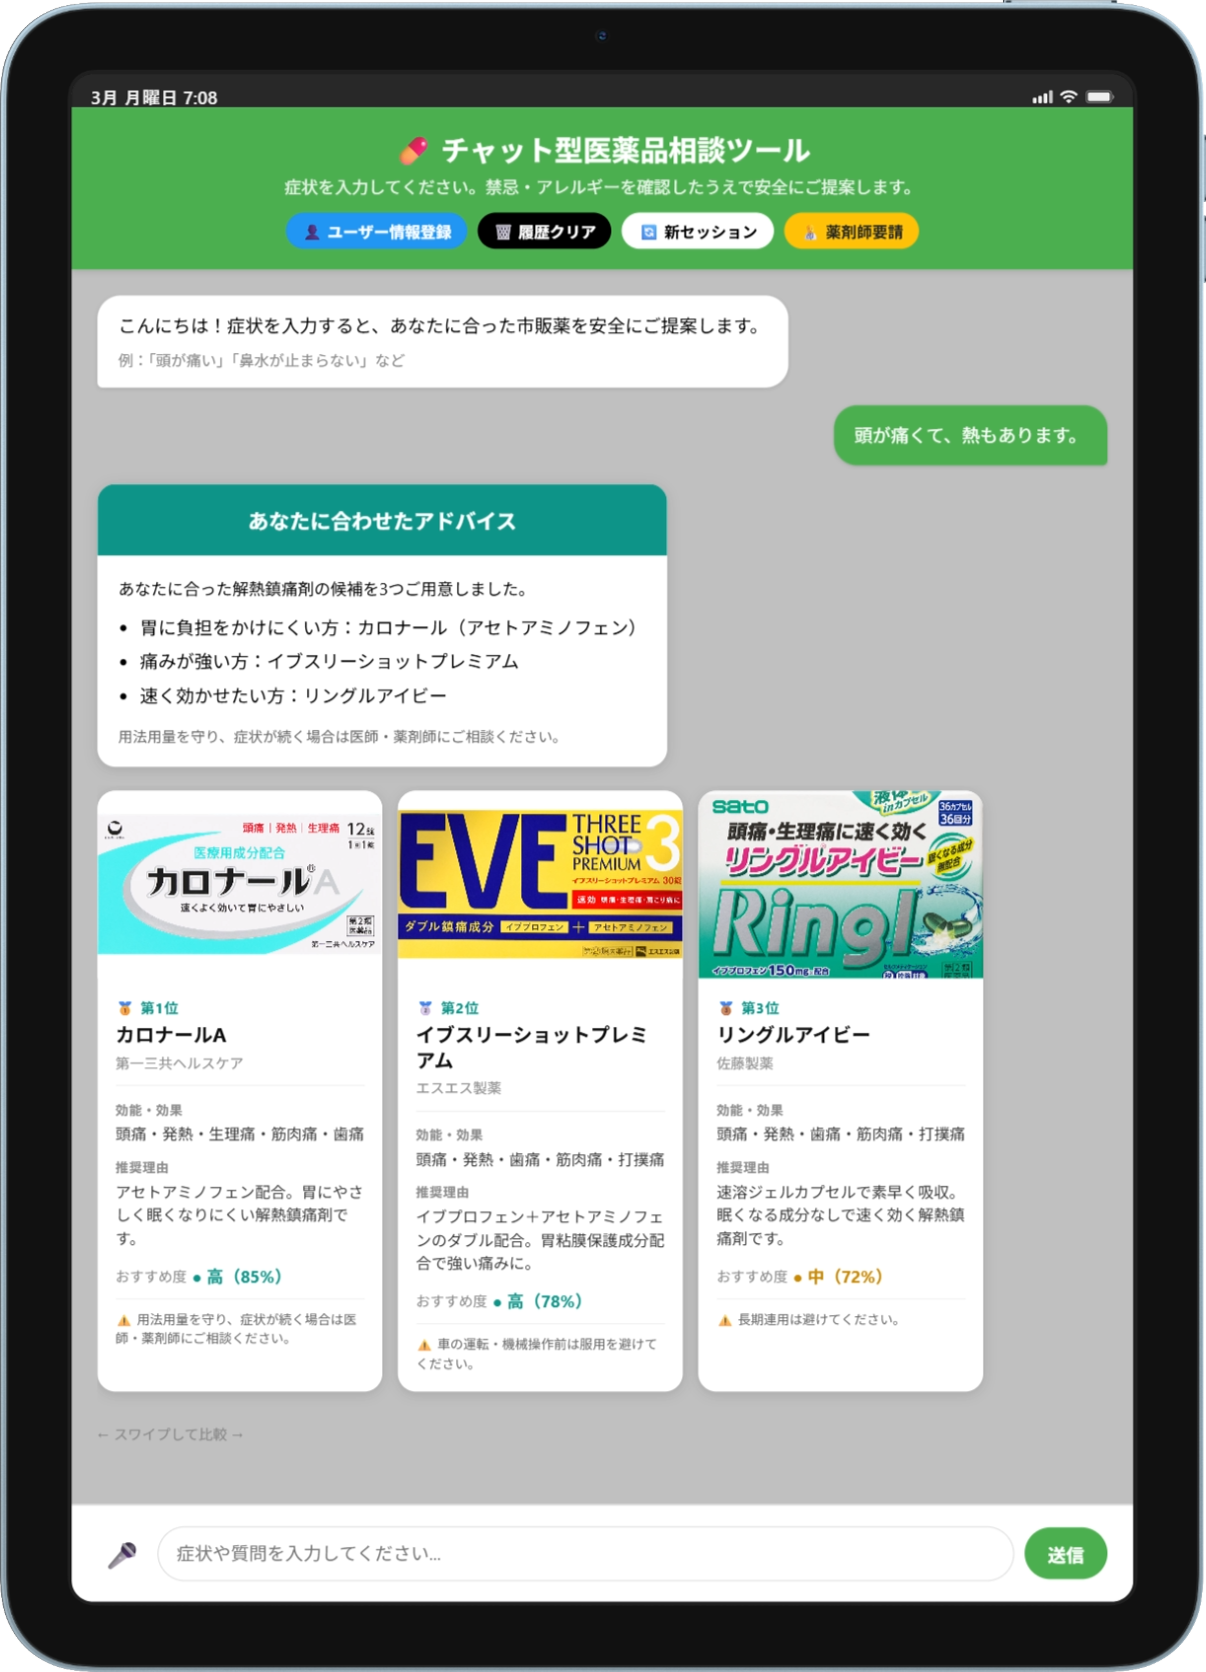
\includegraphics[width=\textwidth,keepaspectratio]{image/carousel_webui.png}
  \caption{Webアプリ版カルーセルUI（未踏期間中に実装）。症状分析・推奨理由・おすすめ度をカード形式で提示する。}
  \label{fig:carousel-webui}
\end{subfigure}
\hfill
\begin{subfigure}[t]{0.45\textwidth}
  \centering
  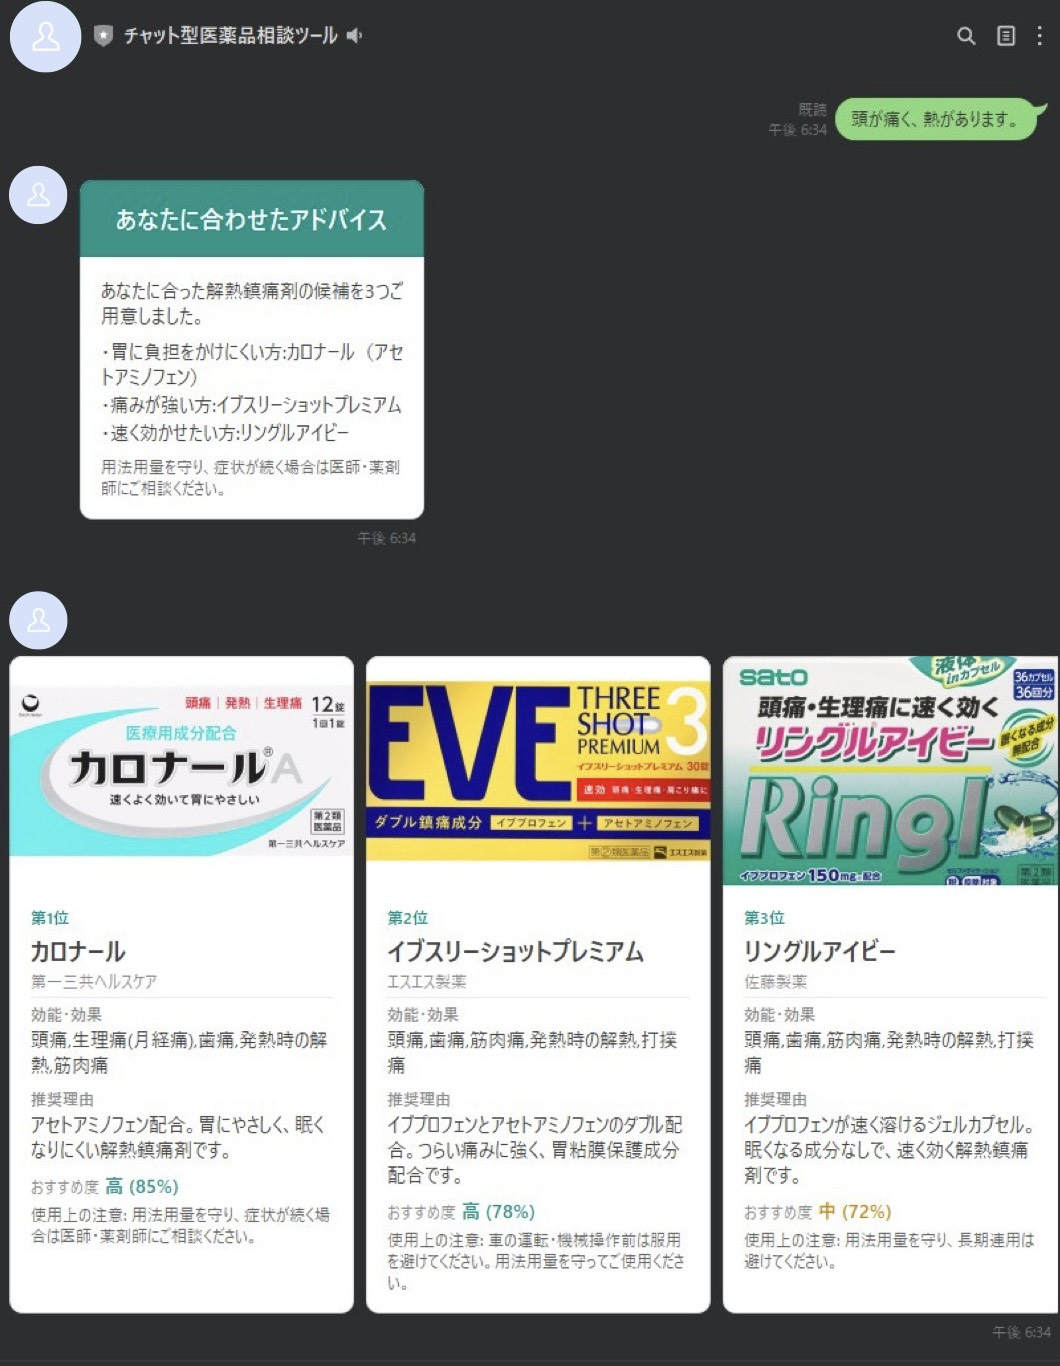
\includegraphics[width=\textwidth,keepaspectratio]{image/line_image.jpg}
  \caption{LINEカルーセル形式による医薬品推奨（中期実装予定）。}
  \label{fig:line-image}
\end{subfigure}
\caption{カルーセル型UIの実装イメージ}
\label{fig:carousel-all}
\end{figure}

\begin{figure}[H]
\centering
\begin{center}
\begin{subfigure}[t]{0.17\textwidth}
  \centering
  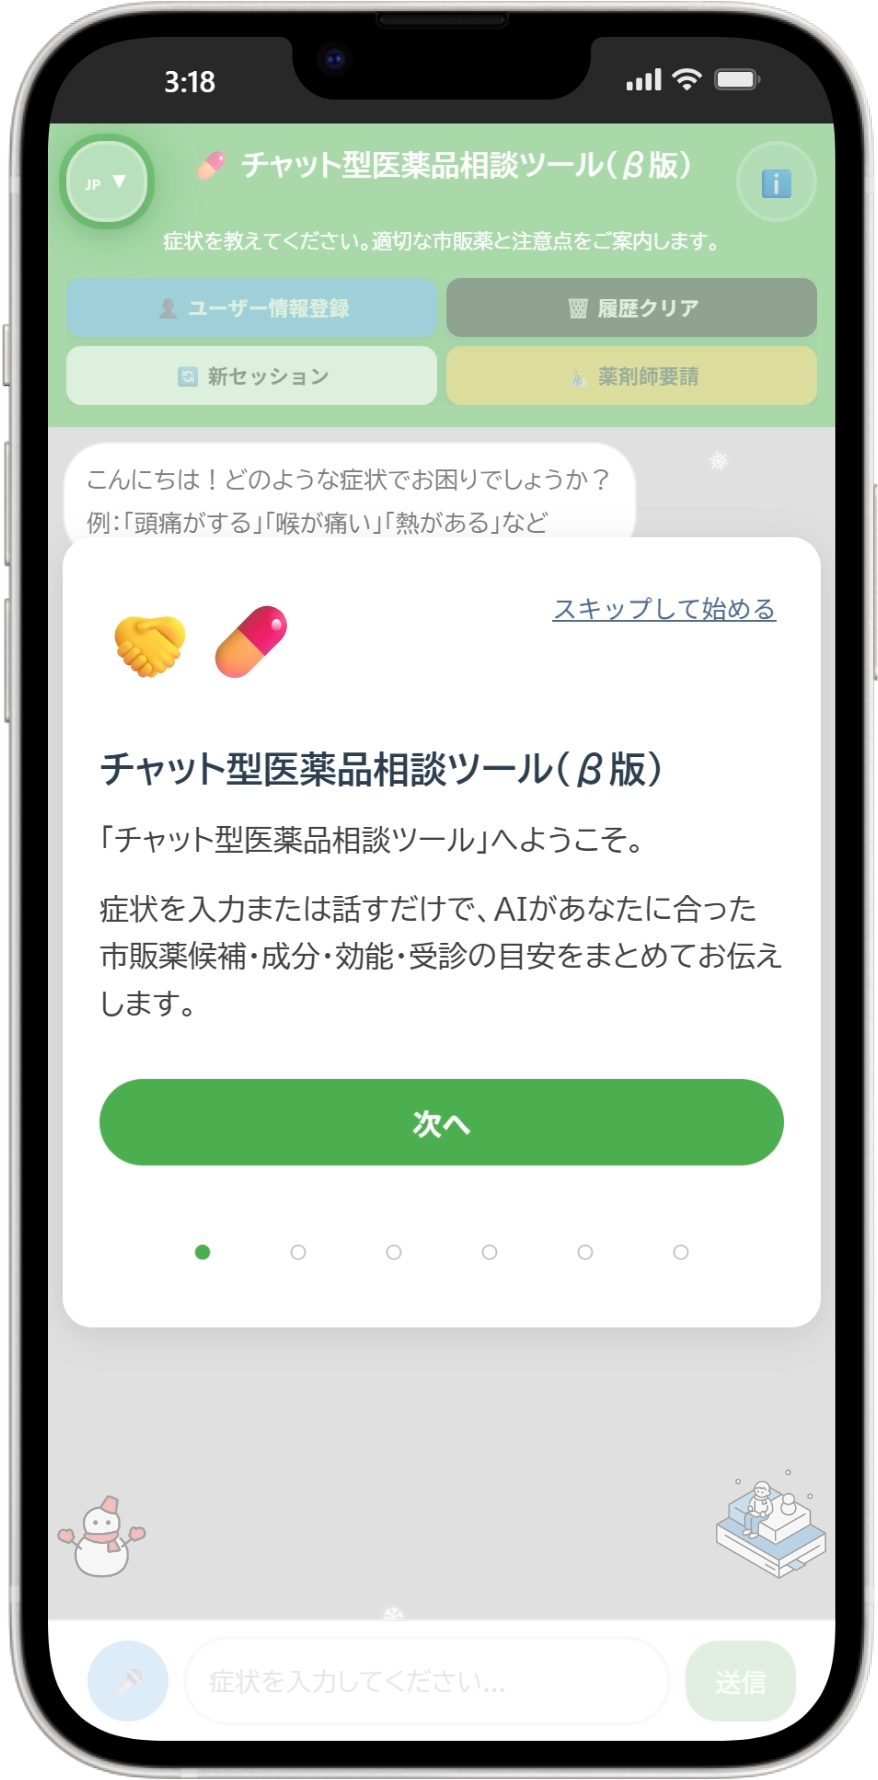
\includegraphics[width=\textwidth,keepaspectratio]{image/onboarding1.png}
\end{subfigure}
\begin{subfigure}[t]{0.17\textwidth}
  \centering
  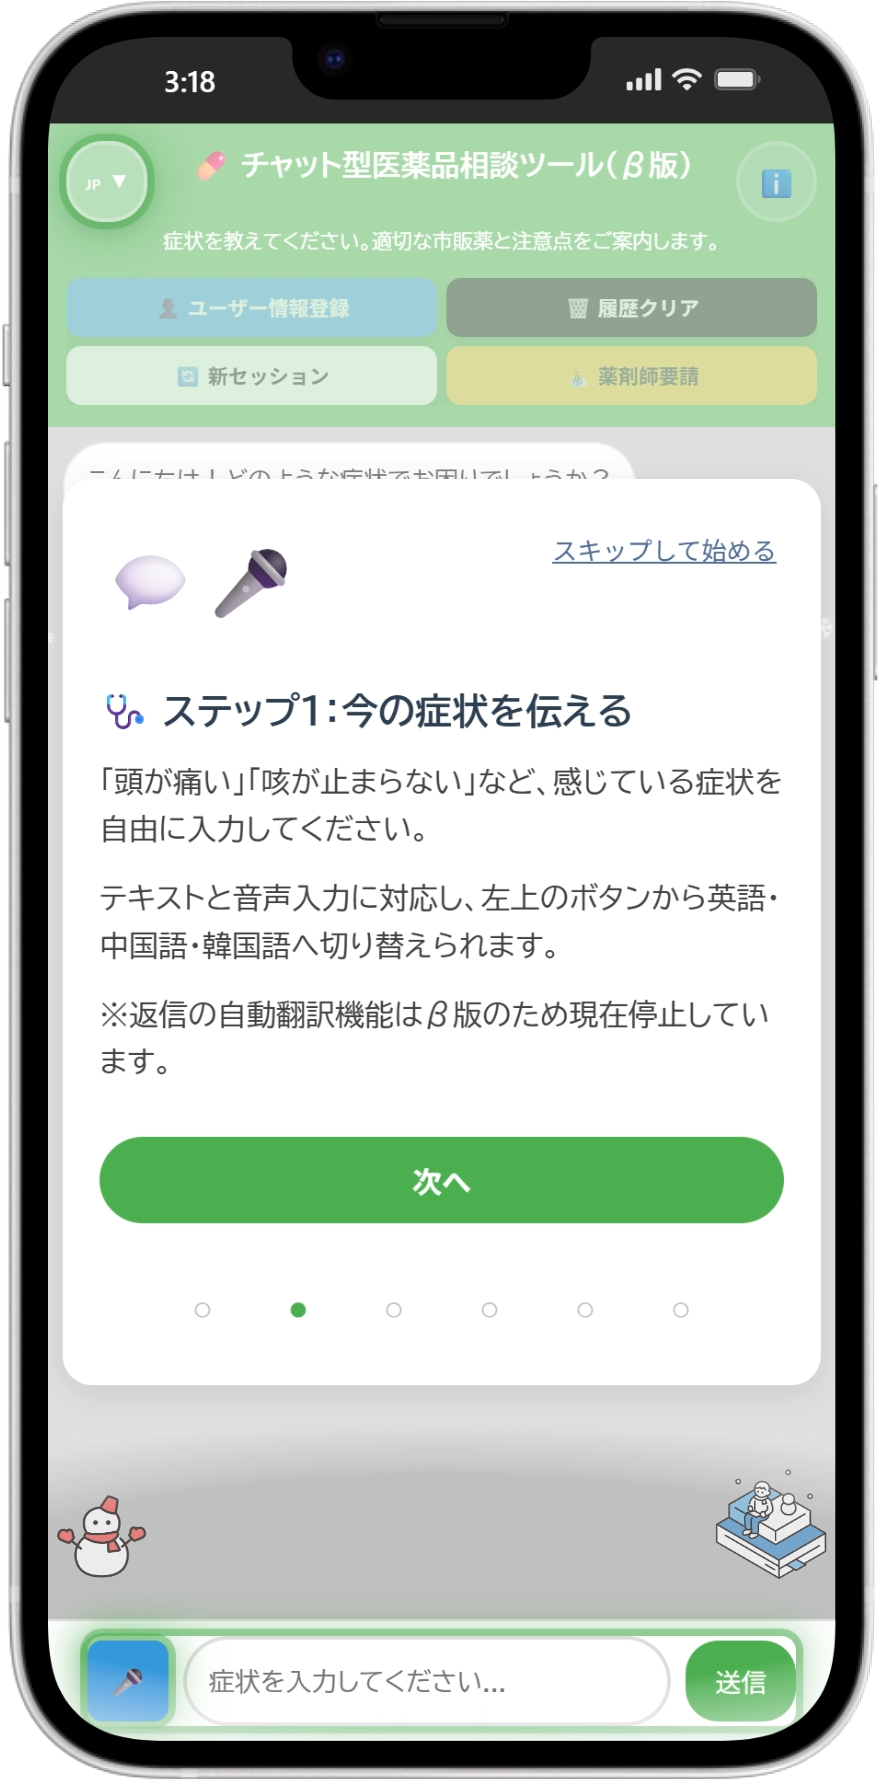
\includegraphics[width=\textwidth,keepaspectratio]{image/onboarding2.png}
\end{subfigure}
\begin{subfigure}[t]{0.17\textwidth}
  \centering
  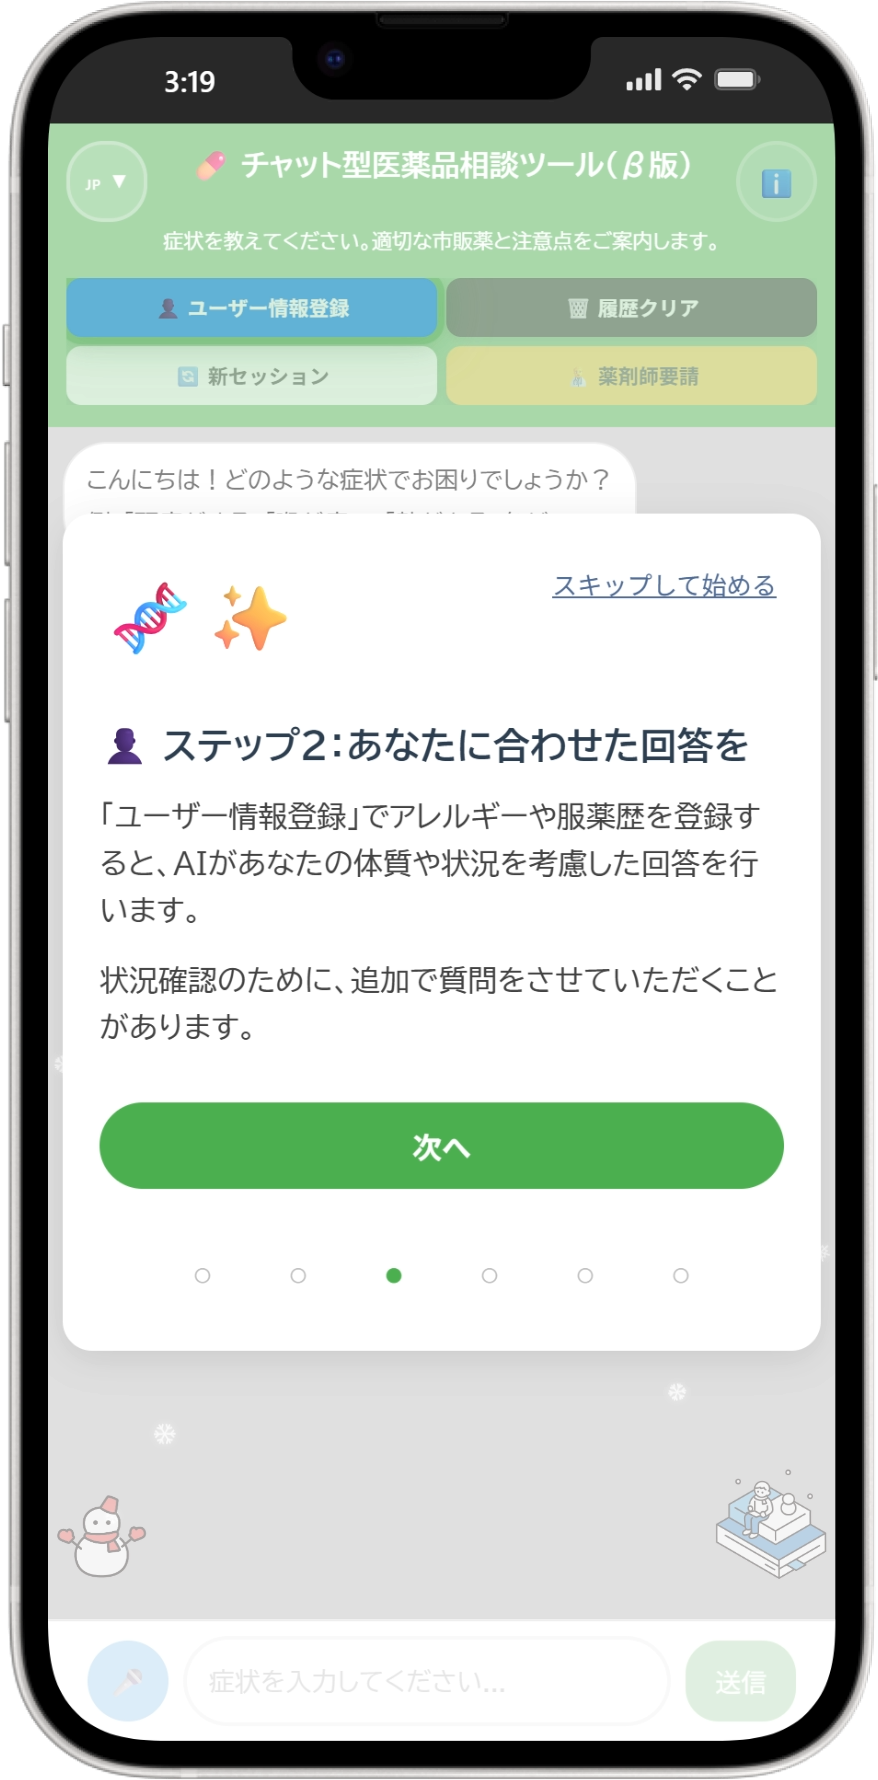
\includegraphics[width=\textwidth,keepaspectratio]{image/onboarding3.png}
\end{subfigure}
\begin{subfigure}[t]{0.17\textwidth}
  \centering
  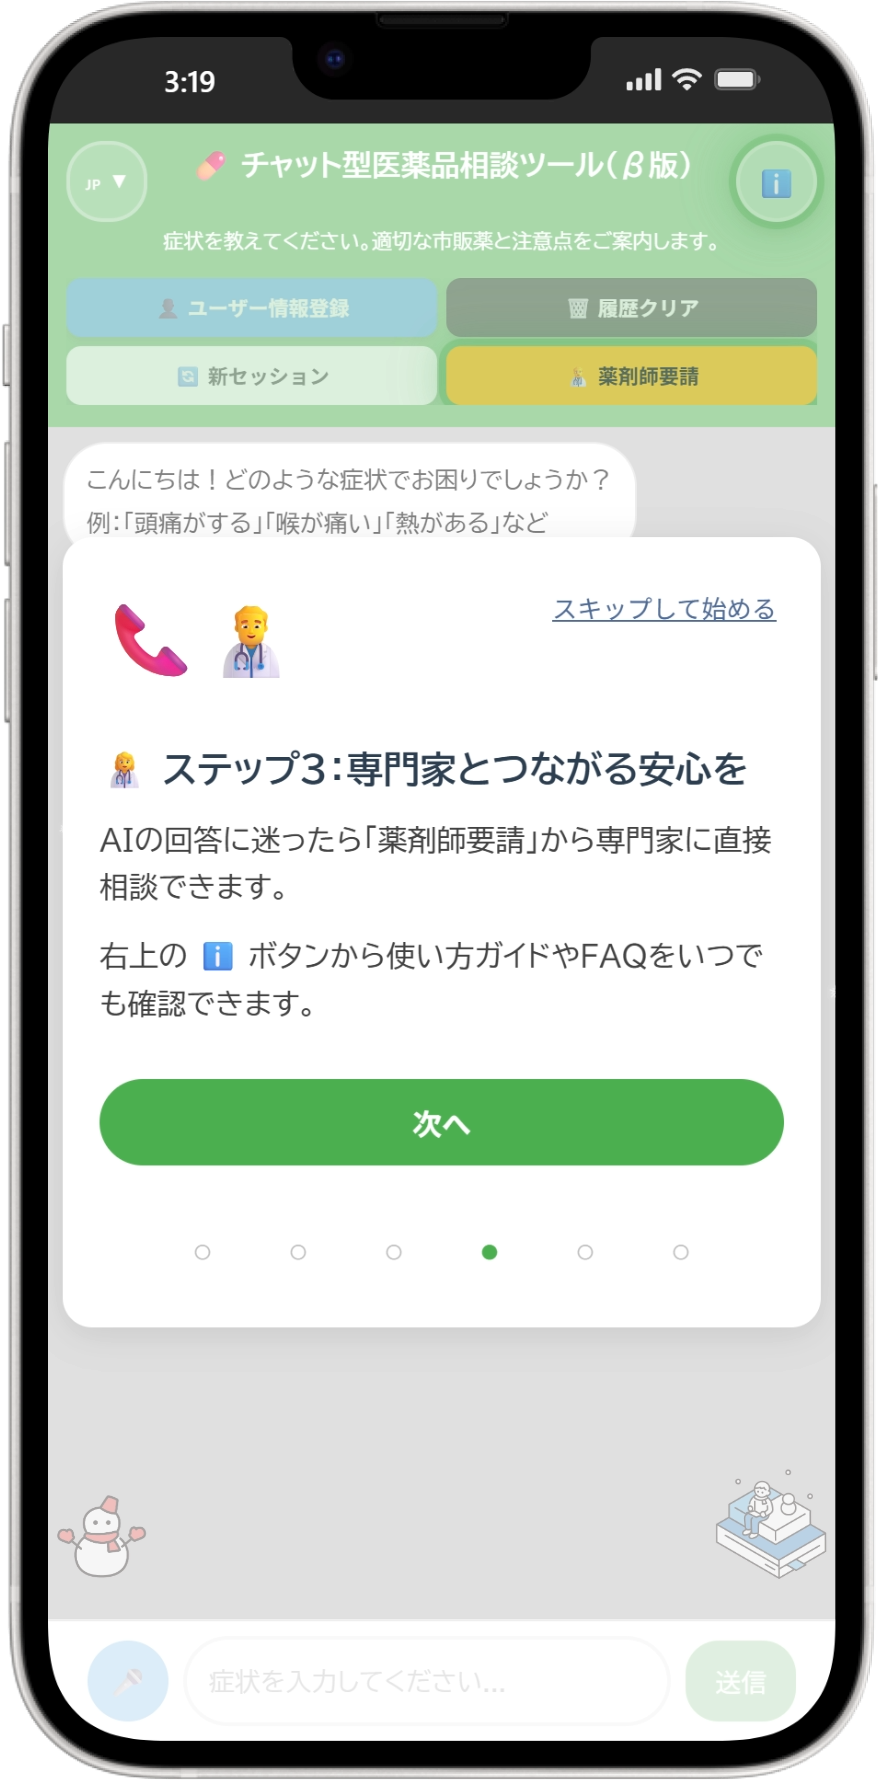
\includegraphics[width=\textwidth,keepaspectratio]{image/onboarding4.png}
\end{subfigure}
\begin{subfigure}[t]{0.17\textwidth}
  \centering
  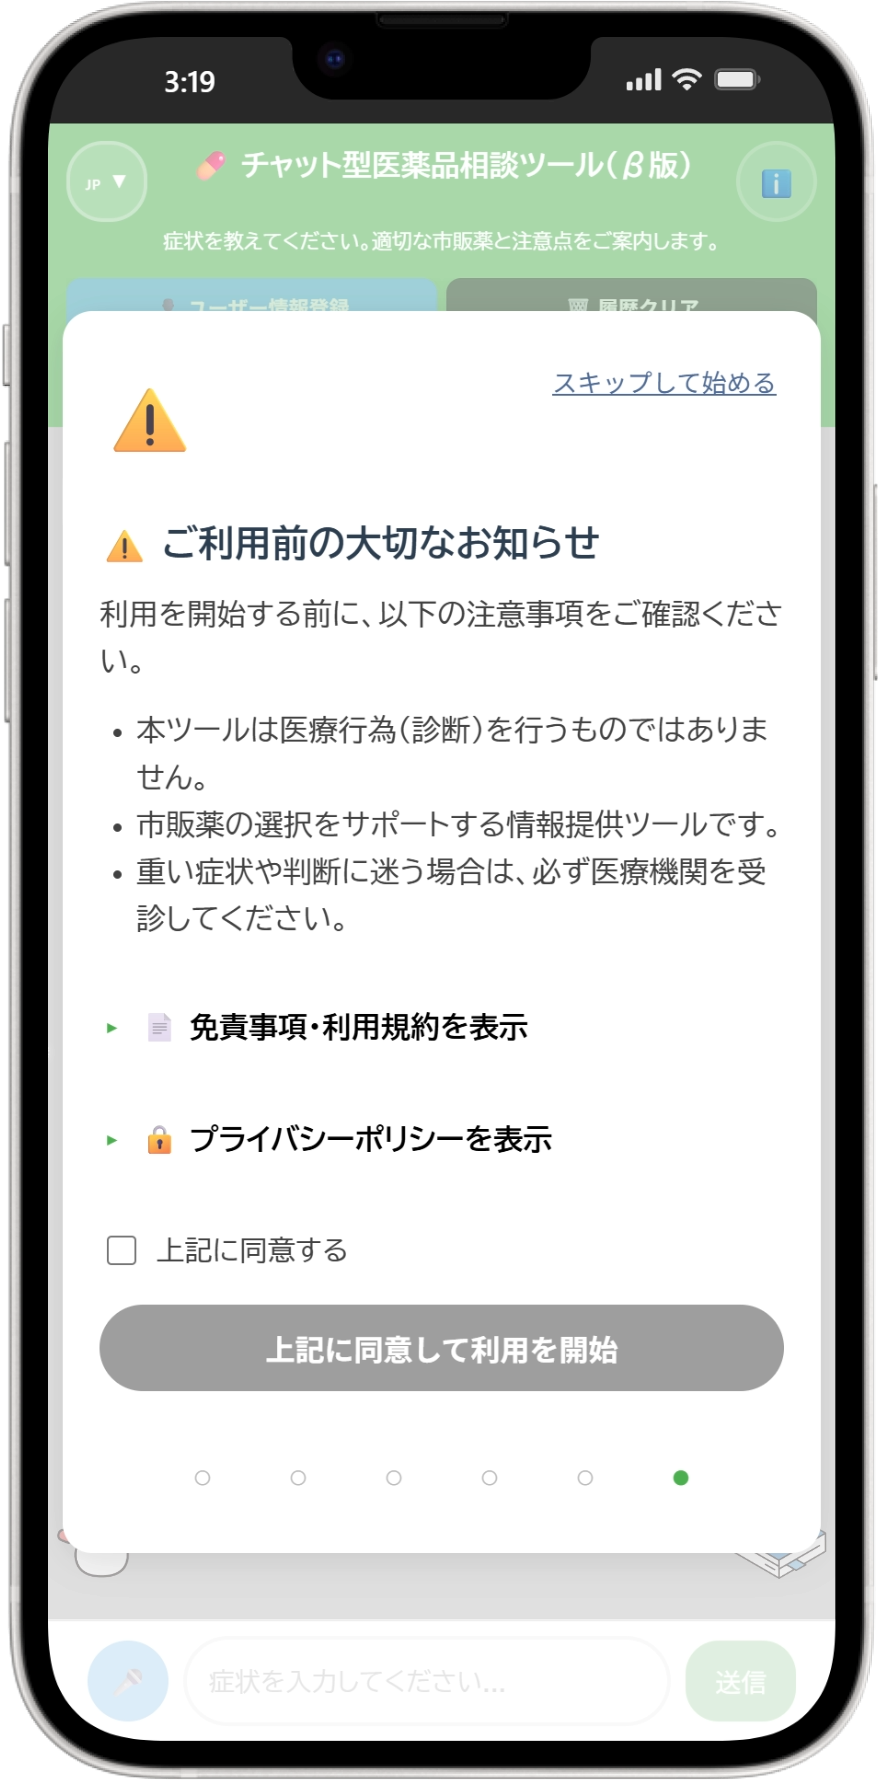
\includegraphics[width=\textwidth,keepaspectratio]{image/onboarding6.png}
\end{subfigure}
\end{center}
\caption{直感的なオンボーディングガイド（言語選択・利用注意・操作案内）\\
音声入力・読み上げ対応により、高齢者や文字入力が苦手な利用者にも配慮している。}
\label{fig:onboarding}
\end{figure}

\begin{figure}[H]
\centering
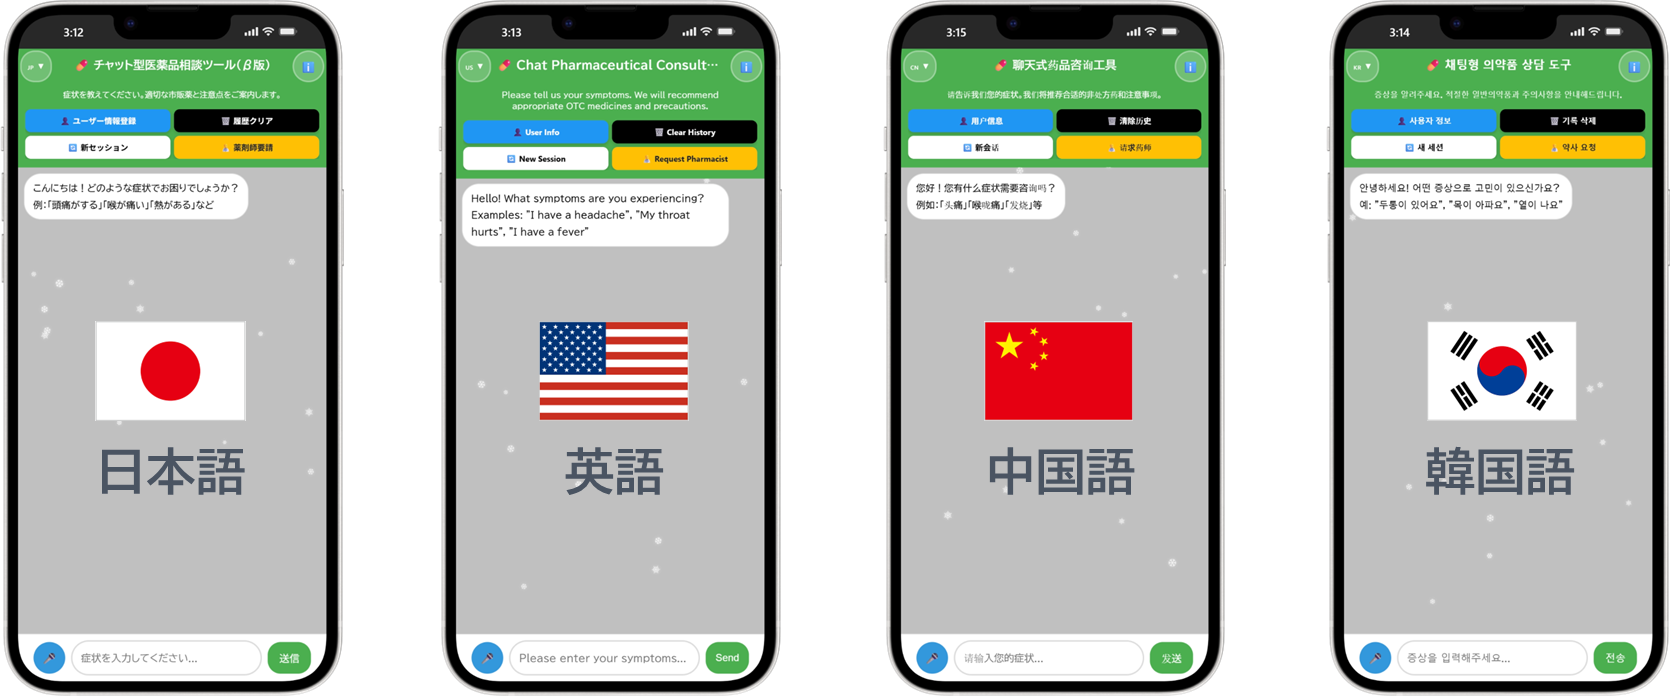
\includegraphics[width=0.85\textwidth,keepaspectratio]{image/language.png}
\caption{対応言語（日本語・英語・中国語・韓国語）の画面例}
\label{fig:language}
\end{figure}

\subsection*{期待される効果}
短期的には、本提案のシステムを通じて、ドラッグストアや自宅など身近な環境から、時間や場所の制約を受けずに医薬品の相談ができるようになる。市販薬選びに不安を抱える利用者に対して、具体的な製品候補と注意点を整理して提示でき、\textbf{相談の質の向上}に寄与する。さらに、図\ref{fig:carousel-all}に示すようにカルーセル型UIによって、推奨された医薬品をパッケージ画像・商品名・効能のカード形式でスワイプしながら確認でき、視覚的に候補を比較できるため、\textbf{推奨結果の認識しやすさと選択への安心感}が向上する。本提案はWebアプリ・LINEチャット・店頭タブレットのいずれにも展開することで、プラットフォームを問わず誰もが「どこでも・安心して」医薬品を選択できる社会を実現する。

中期的には、ユーザーに合った市販薬がわかりやすく提案されることにより、\textbf{市販薬の誤った選択のリスクの低減}が期待される。また、既往症や併用薬を考慮した提案や、市販薬依存のリスクが高い成分を避けるブレーキ機能を日常的な相談フローに組み込まれることで、\textbf{市販薬への薬物依存の低下}にも寄与する。こうした個人レベルの安全性向上が広がることで、適切な市販薬利用の促進と不適正使用の抑制が進み、行政のセルフメディケーション推進施策や、製薬・ドラッグストア業界の適正販売の取り組みを補完する効果が期待される。また、ドラッグストアでは、推奨の質の向上や訪日外国人や多文化環境においても同等の支援を提供でき、\textbf{多言語での公平なアクセス}と店舗スタッフの負担軽減の効果もある。

長期的には、過疎地・離島などで「薬を相談して買う場所がない」という課題の緩和、住む場所による健康格差の縮小、そして適切なセルフメディケーションの普及による\textbf{健康寿命の延伸}や医療機関受診の適正化などが挙げられる。また、本システムによって得られた知見やデータベースは症状の統計やユーザーのニーズに直結し、新薬の開発などにもつながる。専門家の知見をシステムとして共有し、「どこでも・誰にでも同じレベルの説明と提案が届く」状態を実現することで、日本のセルフメディケーションが新しいステージへと進んでいく。

\subsection*{評価指標（どこまで測るか）}
以下の指標は現時点で想定している目標値（目安）であり、テストケース数・データセットの詳細は採択後にPMと相談して確定する。なお、応答時間については既に本番環境（GCP Cloud Run）で稼働中のシステムの実測値をもとに設定している。
\begin{table}[H]
\centering
\caption{評価指標と目標値（目安）}
\label{tab:metrics}
\begin{tabularx}{\linewidth}{llX}
\toprule
種別 & 指標 & 目標・測定方法（目安） \\
\midrule
安全性 & 禁忌判定成功率 & 99\%以上。年齢・妊娠・既往症別のテストケースで検証 \\
安全性 & アレルギー成分検出率 & 99\%（成分単位の網羅的チェック） \\
安全性 & リスク入力ブロック率 & 100\%（プロンプトインジェクション・緊急ワード含む） \\
品質・性能 & 推奨一致率 & 監修者が選んだ推奨との一致率。\\
品質・性能 & 応答時間 & GCP Cloud Run上での実測値30秒以内（OpenAI API呼び出し含む） \\
アクセシビリティ & エラー/再入力率 & 20\%以下（症状入力がリジェクトされ再入力が必要になったセッションの割合。セッションログから自動集計） \\
アクセシビリティ & 多言語完了率 & 85\%以上（英語・中国語・韓国語ユーザーが推奨結果まで到達した割合。言語別セッションログで計測） \\
\bottomrule
\end{tabularx}
\end{table}

% ========== ④ 具体的な進め方と予算 ==========
\section*{\ding{175} 具体的な進め方と予算}

\subsection*{(1) 主に開発を行う場所}
自宅（Windows 11、デスクトップ）および大学・外出先（MacBook Pro、ノートPC）。

\subsection*{(2) 使用する計算機環境（ハード・OS）}
\begin{itemize}[nosep,leftmargin=1em]
  \item \textbf{自宅}：Windows 11 Home、AMD Ryzen 9 9950X（16コア/32スレッド）、メモリ64GB、NVIDIA GeForce RTX 4070 SUPER
  \item \textbf{大学・外出先}：MacBook Pro（2020、Intel Core i7、メモリ16GB、macOS）
\end{itemize}

\subsection*{(3) 使用する言語・ツール}
\begin{table}[H]
\centering
\small
\begin{tabularx}{\textwidth}{@{}lX@{}}
\toprule
カテゴリ & ツール・言語 \\
\midrule
言語・フレームワーク & Python 3.11, Flask 3.x, Gunicorn \\
データベース & PostgreSQL（本番: Neon, 将来的に GCP Cloud SQL も併用検討）, SQLite（開発） \\
API & OpenAI API（GPT-4o-mini：NLU/応答生成, text-embedding-3-small：潜在空間ベクトル生成）, DeepL API \\
インフラ & GCP Cloud Run、GCP Cloud SQL（PostgreSQL、検討中）、Neon（PostgreSQL） \\
\bottomrule
\end{tabularx}
\end{table}

\subsection*{(4) 作業の分担}
個人開発のため、該当なし。

\subsection*{(5) 開発に使う手法}
既存リポジトリをベースとした継続開発。単体・統合・シナリオテストを拡充しつつ、Phase1→2→3 の順で段階的に開発し、各段階で評価可能な状態を維持する。禁忌ルールやフロー設計の妥当性については、薬剤師・登録販売者等の専門家に、8月後半〜12月末の間で2週間に1〜2回程度、一定の完成段階で監修・レビューを依頼する。Phase完了後（未踏期間内）にはよりしっかりとした監修を受け、安全性と現場感覚の両面から検証する予定である。

\subsection*{(6) 開発線表（いつまでに何をするか）}

\begin{figure}[H]
\centering
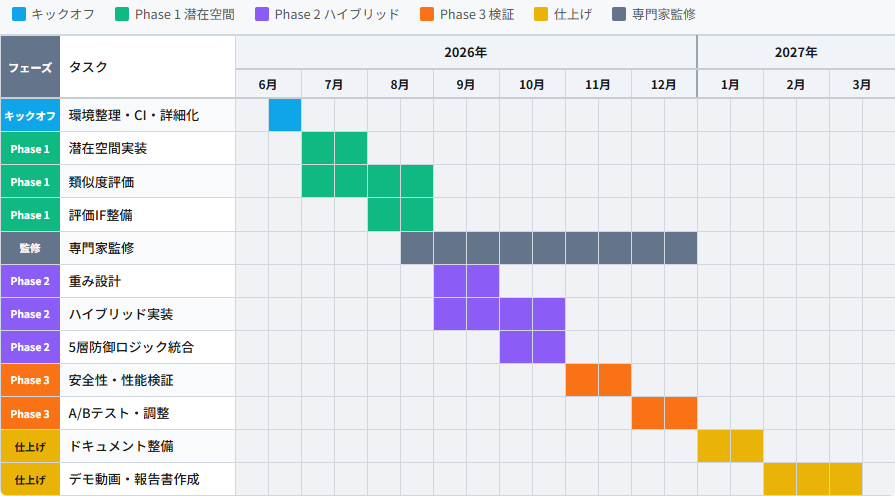
\includegraphics[width=\textwidth,keepaspectratio]{image/gantt_chart.png}
\caption{開発スケジュール（2026.06～2027.03）。Phase2で既存5層防御との結合を完了する。}
\end{figure}

\begin{table}[H]
\centering
\small
\begin{tabular}{@{}c@{\quad}l@{\quad}>{\raggedright\arraybackslash}p{\dimexpr\linewidth-15em\relax}@{}}
\toprule
時期 & 月 & 主な内容 \\
\midrule
開始 & 2026年6月（後半） & 環境・リポジトリ整理、既存テスト・CI確認、9ヶ月計画の詳細化、PM・IPAとのキックオフ \\
第1期 & 7月 & 潜在空間 Phase1: 埋め込みAPI利用設計、約8,000品目の医薬品の埋め込みベクトルをDBに事前計算・保存、コサイン類似度計算の単体テスト通過、ルールベースとの並行評価インターフェース動作確認まで完了。（\refmark 7月末は試験のため開発少なめ） \\
第2期 & 8月 & \textbf{【Phase1 完了】}上記の成果物の達成を確認後、評価用データ・シナリオの整備。Phase2 設計（重み・動的重み付け） \\
専門家監修 & 8月後半～1月末 & 2週間に1〜2回程度、一定の完成段階で薬剤師・登録販売者等に監修・レビューを依頼。Phase完了後にしっかりとした監修を受ける。 \\
第3期 & 9月 & Phase2: ハイブリッドスコアリング関数の実装、既存5層防御との結合、統合テスト一式通過。\textbf{【Phase2 完了】}既存安全性指標（禁忌99\%・アレルギー98\%）を確認。 \\
第4期 & 10月 & 安全性検証（禁忌・アレルギー検出率の維持）、パフォーマンス・レイテンシ確認、不具合修正 \\
第5期 & 11月 & Phase3: 監修テストケースでルールベース単体との推奨一致率を比較。パラメータ設定根拠を含む評価レポートを提出可能な状態に完成。\textbf{【Phase3 完了】} \\
第6期 & 12月 & ドキュメント整備（技術文書・README）、運用周り改善 \\
第7期 & 2027年1月 & 残タスク消化、デモ・動画の準備、成果報告書の下書き（\refmark 1月末は試験のため開発少なめ） \\
終了 & 2月～3月12日 & 成果報告書・実績報告書の取りまとめ、提出物の最終確認 \\
\bottomrule
\end{tabular}
\end{table}

\subsection*{(7) 開発にかかわる時間帯と時間数}
開発時間帯は、平日は放課後〜夜、土日祝は午前〜夕方を中心に確保する。開発期間は2026年6月22日～2027年3月12日（約9ヶ月）とする。試験期は7月末1週・1月末3週の計4週で週15時間、計60時間とする。夏休み期は8月第2週～9月末の54日で1日8時間、計432時間とする。通常期はそれ以外の平日120日・土日祝62日とし、平日3時間/日、土日祝8時間/日で計856時間とする。以上、\textbf{合計 1,348時間}を申請する（上限1,440時間以内）。内訳は下表のとおりである。

\begin{table}[H]
\centering
\small
\begin{tabular}{@{}llrr@{}}
\toprule
期間 & 内容 & 1日あたり時間 & 小計（時間） \\
\midrule
試験期（4週） & 7月末1週、1月末3週 & 週15時間 & 60 \\
夏休み期 & 8月第2週～9月末（54日） & 7h/日 & 432 \\
通常期 & 平日120日・土日祝62日 & 平日3h/日、土日祝8h/日 & 856 \\
\midrule
\multicolumn{3}{r}{合計} & 1,348 \\
\bottomrule
\end{tabular}
\end{table}

\subsection*{(8) 予算内訳}
申請金額は、1,348時間 × 2,100円/時間（税抜）＝ \textbf{2,830,800円}（税抜）とする。下表の必要経費はプロジェクト遂行に充てる目安である。

\begin{table}[H]
\centering
\begin{tabularx}{\linewidth}{l>{\raggedright\arraybackslash}Xr}
\toprule
費目 & 内容 & 概算（円） \\
\midrule
OpenAI API & 埋め込み・LLM呼び出し（開発・検証・本番） & 80,000～100,000 \\
DeepL API & 多言語応答用（開発・検証・本番環境） & 10,000～20,000 \\
GCP・Neon & Cloud Run・Cloud SQL（PostgreSQL）、Neon（PostgreSQL）利用料（開発・本番） & 10,000～25,000 \\
専門家監修 & 薬剤師・登録販売者等による内容監修・レビュー謝礼（8月後半～1月末で2週間に1～2回程度、Phase完了後にしっかりとした監修を受ける） & 80,000～200,000 \\
書籍・文献 & 機械学習・NLP・医薬品・セキュリティ関連 & 15,000～25,000 \\
ドメイン・その他 & ドメイン更新、開発用ツール等 & 10,000～30,000 \\
\bottomrule
\end{tabularx}
\end{table}

実際の支出は作業進捗に応じて行い、実績報告書で報告する。

% ========== ⑤ 提案者の腕前 ==========
\section*{\ding{176} 提案者（たち）の腕前を証明できるもの}

\begin{itemize}[nosep]
\begin{bodyminipage}[c]{0.75\linewidth}
\item \textbf{本システム}:医薬品推奨システムを個人で設計・開発し、公開運用中（\url{https://medicine.yutok.dev/}）。GitHubリポジトリ：\url{https://github.com/32Lwk/medicine-recommend-system}。本システムの設計・実装はすべて自分で行った。5層防御・ルールベーススコアリング・ハイブリッドNLU（辞書＋LLMフォールバック）を実装済み。4言語対応、GCP Cloud Run・Neon（PostgreSQL）本番運用の実績あり。未踏期間では、潜在空間の設計・実装と評価を新規に実施する。
\item \textbf{技術スタック}: Python、TypeScript、HTML/CSS、JavaScript、C、PostgreSQL、OpenAI API を本プロジェクトおよび個人開発で用いている。登録販売者資格を2025年10月に取得しており、現場で得た知見をルール設計・用語選定に反映している。
\end{bodyminipage}\hfill
\begin{minipage}[c]{0.22\linewidth}
\centering

\includegraphics[width=\linewidth,keepaspectratio]{image/Demo.png}
\captionof{figure}{本システムのデモ（\url{https://medicine.yutok.dev/}）}
\end{minipage}
\item \textbf{受賞歴}：
\begin{itemize}[nosep,leftmargin=1em]
\item \makebox[9em][l]{2022年7月}（高校時代）：缶サット甲子園 和歌山大会 優勝
\item \makebox[9em][l]{2022年12月}（高校時代）：きのくにプログラミングコンテスト 最優秀賞
\item \makebox[9em][l]{2025年2月}：AWSデジタル社会実現ツアー2025 名古屋本戦 本戦出場
\item \makebox[9em][l]{2025年11月}：ユメカタリ 学生生成AIコンテスト 最優秀賞
\item \makebox[9em][l]{2025年12月}：椙山女学園大学第13回ビジネスコンペティション 優秀賞
\item \makebox[9em][l]{2025年12月}：第9回和歌山県データ利活用コンペティション クオリティソフト賞
\item \makebox[9em][l]{2026年1月}：doda アイデアコンペティション 審査員特別賞
\end{itemize}
\item \textbf{資格}: 基本情報技術者、登録販売者。
\end{itemize}

% ========== ⑥ 特記事項 ==========
\section*{\ding{177} プロジェクト遂行にあたっての特記事項}

\begin{itemize}[nosep]
\item \textbf{学業との両立}: 名古屋大学理学部物理学科2年生（在学中）。指導教員はいない。学業との両立は自己管理で対応する。2年生のため研究室には未配属であり、在籍研究室は該当しない。
\item \textbf{組織・上司}: 該当なし（学生・個人開発）。
\item \textbf{進学・就職・転職・転居}: 開発期間中は特になし。
\item \textbf{チーム}: 個人開発のため、該当なし。
\item \textbf{未成年・保護者}: 該当なし（成年）。
\item \textbf{PM・IPAへの要望・固有の事情}: 特になし。
\item 提案書作成にあたり、文章の推敲のために生成AIを利用した。
\end{itemize}

% ========== ⑦ IT以外 ==========
\section*{\ding{178} IT以外の勉強、特技、生活、趣味など}

\textbf{勉強}: 専攻は物理学・宇宙物理学である。松原隆彦著「宇宙のかたち」を読み、夜空に一様に広がって見える星々にも実は奥行きがあり、銀河が連なってできた銀河フィラメントや、銀河がほとんど存在しないボイドなどの大規模構造が宇宙に広がっていることを知った。そのスケールの大きさと構造の神秘に強く惹かれ、宇宙物理学を志した。大学進学時には情報系学科も候補にあったが、まずは自然現象を支える数理やモデル化を軸に宇宙を理解したいと考え、理学部物理学科を選択した。物理学を通して培った、現象をモデル化しデータから構造を読み取る姿勢は、本プロジェクトにおける医薬品データ設計やルール構築にも活きている。将来的には観測データ解析や機械学習を用いた宇宙構造研究にも取り組みたいと考えている。

\textbf{特技・スポーツ}: 中学では軟式テニス部、高校では硬式テニス部に所属していた。長く競技を続ける中で、小さな改善の積み重ねが大きな成果につながることを体感した。現在はランニングを日課としており、勉強や開発で思考が行き詰まったときに走ることで気持ちを整理している。走っている最中にプロジェクトのアイデアや実装方針が浮かぶことも多く、思考を整える大切な時間になっている。

\textbf{生活で大切にしていること}: 相手の立場に立って考え、安心感を与える行動である。登録販売者として勤務する中で、専門知識を一方的に伝えるのではなく、相手の困りごとを丁寧に汲み取り、理解しやすい言葉で説明することを常に意識している。

\textbf{趣味}: 散歩、ランニング、一人で考え事をする時間である。歩いたり走ったりしながら物事を考える時間が、自分にとって最も思考が整理される時間である。

% ========== ⑧ 将来のIT ==========
\section*{\ding{179} 将来のITについて思うこと・期すること}
宇宙物理学では、目に見えない暗黒物質が銀河の大規模構造を支えているように、社会にも人の判断を静かに支えている「見えない構造」が存在する。近年の機械学習や生成AIにおける潜在空間は、言葉や知識の背後にあるその構造を、データの中から浮かび上がらせる試みだと感じている。宇宙で直接見えない構造を観測から推定するように、ことばや知識の背後にある構造に触れられることに、ITのおもしろさを感じている。

一方で、ITが社会インフラへと深く入り込むほど、その「見えない構造」をブラックボックスのまま社会に委ねてよいのかという問題も生じる。医療、金融、交通、行政など、設計の良し悪しが安全や人生に直結する領域では、スピードや新規性だけでなく、誤らないこと、説明できること、止まらないことがより強く求められる。生成AIによって実装のハードルは確かに下がったが、その一方で「どこまでを機械に任せ、どこを人が責任を持つのか」という設計判断の重要性はむしろ高まっているように思う。

本提案で目指している、誤りを防ぎつつ説明可能な医薬品選択支援システムの設計は、その一つの実践例である。ITが単なる便利な道具にとどまらず、人が安心して判断できる環境を静かに支える存在になることが、これからのITには重要だと考えている。

宇宙の大規模構造が重力によって長い時間をかけて形づくられるように、社会の信頼もまた、堅実な設計と運用の積み重ねによって形成される。将来のITには、新しい可能性を切り拓く力と同時に、人が安心して任せられる基盤であり続けることを期待している。未踏は、技術だけでなく思想まで実装しようとする人間が集まる、稀有な場所だと感じている。もしその一員として挑戦する機会をいただけるなら、ここでしか生まれないような試行錯誤を通して、自分なりの技術を形にしてみたい。

\end{document}
